%% LaTeX2e class for student theses
%% thesis.tex
%% 
%% Karlsruhe Institute of Technology
%% Institute for Program Structures and Data Organization
%% Chair for Software Design and Quality (SDQ)
%%
%% Dr.-Ing. Erik Burger
%% burger@kit.edu
%%
%% See https://sdq.kastel.kit.edu/wiki/Dokumentvorlagen
%%
%% Version 1.6, 2024-06-07

%% Available page modes: oneside, twoside
%% Available languages: english, ngerman
%% Available modes: draft, final (see README)
\documentclass[twoside, english]{sdqthesis}

%% ---------------------------------
%% | Information about the thesis  |
%% ---------------------------------

%% Name of the author
\author{Robin Schulz}

%% Title (and possibly subtitle) of the thesis
\title{Integration of Triple Graph Grammars in Vitruvius}

%% Type of the thesis 
\thesistype{Master's Thesis}

%% Change the institute here, ``KASTEL'' is default
% \myinstitute{Institute for \dots}

%% You can put a logo in the ``logos'' directory and include it here
%% instead of the SDQ logo
% \grouplogo{myfile}
%% Alternatively, you can disable the group logo
% \nogrouplogo

%% The reviewers are the professors that grade your thesis
\reviewerone{Prof. Dr. Ralf Reussner}
\reviewertwo{Prof. Dr.-Ing. Anne Koziolek}

%% The advisors are PhDs or Postdocs
\advisorone{Lars König, M.Sc.}
%% The second advisor can be omitted
\advisortwo{Thomas Weber, M.Sc.}

%% Please enter the start end end time of your thesis
\editingtime{18 November 2024}{18 May 2025}

%% Please enter the place of residence of the author. This is used on the declarationpage
\location{Karlsruhe}

\settitle

%% --------------------------------
%% | Bibliography                 |
%% --------------------------------

%% Use biber instead of BibTeX, see README
\usepackage[citestyle=numeric,style=numeric,backend=biber]{biblatex}
\addbibresource{thesis.bib}

% Suppress URL if DOI is present
\renewbibmacro*{doi+eprint+url}{%
  \iftoggle{bbx:doi}
    {\printfield{doi}}
    {}%
  \newunit\newblock
  \iftoggle{bbx:eprint}
    {\usebibmacro{eprint}}
    {}%
  \newunit\newblock
  \iftoggle{bbx:url}
    {\iffieldundef{doi}{\usebibmacro{url+urldate}}{}}
    {}}

%% For example texts -- please remove in the final version
\usepackage{blindtext}

% TODOnotes - the following is required for it to work, remove for final!
\setlength {\marginparwidth }{2cm}
\usepackage{todonotes}
\usepackage{listings}
\usepackage{float}
\usepackage{algpseudocode}
\usepackage[chapter]{algorithm}

\usepackage{amsmath}
% for listings
\usepackage{xcolor}

\usepackage{multirow}
\usepackage{makecell}

\usepackage{pgfplots} 
\pgfplotsset{compat=1.18}

\definecolor{codegreen}{rgb}{0,0.6,0}
\definecolor{codegray}{rgb}{0.5,0.5,0.5}
\definecolor{codepurple}{rgb}{0.58,0,0.82}
\definecolor{backcolour}{rgb}{0.95,0.95,0.92}

\lstdefinestyle{mystyle}{
    backgroundcolor=\color{backcolour},   
    commentstyle=\color{codegreen},
    keywordstyle=\color{magenta},
    numberstyle=\tiny\color{codegray},
    stringstyle=\color{codepurple},
    basicstyle=\ttfamily\footnotesize,
    breakatwhitespace=false,         
    breaklines=true,                 
    captionpos=b,                    
    keepspaces=true,                 
    numbers=left,                    
    numbersep=5pt,                  
    showspaces=false,                
    showstringspaces=false,
    showtabs=false,                  
    tabsize=2
}

\lstset{style=mystyle}

% GQM-Liste
\newlist{gqm}{enumerate}{3}
\setlist[gqm,1]{label={G\arabic*}}
\setlist[gqm,2]{label={Q\arabic{gqmi}.\arabic*}}
\setlist[gqm,3]{label={M\arabic{gqmi}.\arabic{gqmii}.\arabic*}}

%% ====================================
%% ====================================
%% ||                                ||
%% || Beginning of the main document ||
%% ||                                ||
%% ====================================
%% ====================================
\begin{document}

%% Set PDF metadata
\setpdf

%% Set the title
\maketitle

%% The Preamble begins here
\frontmatter

\input{sections/declaration.tex}

\setcounter{page}{1}
\pagenumbering{roman}

%% ----------------
%% |   Abstract   |
%% ----------------
 
%% For theses written in English, an abstract both in English
%% and German is mandatory.
%%
%% For theses written in German, a German abstract is sufficient.
%%
%% The text is included from the following files:
%% - sections/abstract

\includeabstract

%% ------------------------
%% |   Table of Contents  |
%% ------------------------
\tableofcontents

\listoffigures
\listoftables

%% -----------------
%% |   Main part   |
%% -----------------

\mainmatter

%% LaTeX2e class for student theses
%% sections/content.tex
%% 
%% Karlsruhe Institute of Technology
%% Institute for Program Structures and Data Organization
%% Chair for Software Design and Quality (SDQ)
%%
%% Dr.-Ing. Erik Burger
%% burger@kit.edu
%%
%% Version 1.6, 2024-06-07

\chapter{Introduction}
\label{ch:Introduction}

The development of many large modern IT systems and cyber-physical systems (CPS) is characterized by the use of different languages and tools to describe different parts and aspects of the system under development, e.g., design, implementation, and documentation and different subdomains and subsystems. The use of different languages produces different informational artifacts describing the system and dependencies between those artifacts.

As an approach to cope with increasingly complex conglomerates of different artifacts that all describe a single system, \emph{Model Driven Engineering} (MDE) \cite{kent_model_2002} has become a strategy with industrial relevance \cite{hutchinson_model-driven_2011, hutchinson_model-driven_2014, whittle_state_2014}.
In the software context, different groups of developers of such systems can form by assigning different roles to software developers or by choosing certain architectural patterns or development processes. Examples of such roles are software architects, system deployers, and component developers. Systems that not only consist of software introduce further groups of developers, e.g., electrical or mechanical engineers, that also produce artifacts that describe the system from physical viewpoints.
To account for different perspectives and concerns, in short: for viewpoints, that different groups of developers have, the view-based paradigm has been established. Here, various views are defined that represent partial information of a system that is relevant from the viewpoint of the roles that different developer groups assume.
With the usage of multiple models that constitute a system, these models often share information, which introduces redundancy, and the question of how to prevent that redundancy or keep redundant information consistent arises.
Klare et al. \cite{VitruviusKlare2021} aim to answer that question by proposing the concept of \emph{Virtual Single Underlying Model}s (V-SUMs) and presenting the \textsc{Vitruvius} approach.
Aiming to combine \enquote{the advantages of synthetic and projective modeling}  \cite{VitruviusKlare2021}, the projective concept of a view as a dynamically generated model is combined with the synthetic concept of describing the system with multiple interrelated models instead of one. The concepts of projective and synthetic views are defined in the ISO 42010 standard \cite{iso_42010}.
With V-SUMs, developers only use views to modify the system.
To be able to keep the system in a consistent state, \emph{consistency preservation rules} (CPRs) are defined.
They specify how consistency is preserved between models and are executed if changes are made to one model. 
Alongside view definition languages, languages that are specialized for consistency preservation play the key role in keeping consistency between the models that form the system description of a V-SUM.

While such languages exist and have been implemented for V-SUMs in the context of \textsc{Vitruvius}, there are also existing and mature \cite{fritsche_short-cut-theoretical_2018, fritsche_higher_order_short_cut_rules_2023} general-purpose model-transformation languages that are able to express complex relations between models. One such concept is given by \emph{Triple Graph Grammars} (TGGs) \cite{schurr_tggs_1995}, which consist of context-sensitive graph production rule patterns that relate a pair of graphs by building a third graph representing the relation. These rules can be used for keeping two models consistent in an incremental manner via pattern matching.
% This allows for minizmizing data loss and improving performance, because. 

TGGs allow for specifying descriptive rules that can concern any number of entities, and the graph approach allows for graphical visualization of these potentially complex relations. To use that advantage for consistency preservation in V-SUMs and examine the resulting approach, the following research questions are answered in this thesis:
\begin{enumerate}
    \item How can TGG rules be applied in delta-based consistency preservation processes?
    \item What kinds of consistency relations can be expressed with the developed concept?
\end{enumerate}

To that end, the aim of this thesis is to investigate how TGGs can be used for consistency preservation in \textsc{Vitruvius} by researching how sequences of \textsc{Vitruvius} changes can be converted to sequences of TGG rule applications. This is done by elaborating a concept, and developing a prototype that implements that concept.

This concept, which is called \emph{Backward Conversion Pattern Matching}, is explained in \autoref{ch:Concept}. In addition to the process of converting TGG rules to something that is matchable to sequences of \textsc{Vitruvius} changes and the matching process, several additional process steps are necessary to make the concept realizable, such as handling deleting changes (\autoref{sec:Concept:RedMatching}) or context matching (\autoref{alg:BackwardConversionPM:BlackMatching}).
Details of the prototype implementation of the elaborated concept are described in extracts in \autoref{ch:Implementation}.
The evaluation of the concept via the prototype is shown in \autoref{ch:Evaluation}, as well as a discussion of the results.
In \autoref{ch:RelatedWork}, a brief overview of work related to the thesis is given, mainly presenting other approaches to consistency preservation.
Chapter \ref{ch:Conclusion} concludes by summarizing the work done in the thesis, the evaluation results and their discussion, and giving an outlook to future research related to this work.
\chapter{Foundations}
\label{ch:Foundations}
This chapter provides an overview of the theoretical and practical foundations of \emph{Virtual Single Underlying Models} (V-SUMs), model-driven software engineering, model synchronization, and Triple Graph Grammars.

\section{Model-Driven Software Engineering}
\label{sec:Foundations:MDSE}
Model-driven software Engineering (MDSE), or sometimes referred to as model-driven software development (MDSD), is an approach to software engineering that Kramer \cite{kramer_specification_2017} describes as
\enquote{a development paradigm in which models are used in an automated way for all development tasks}.
Well-known approaches to this paradigm are the Object Managment Group's Model-Driven Architecture (MDA) approach \cite{model_driven_architecture_omg} and the  Unified Modeling Language \cite{OMG_UML_2.5.1}, the latter being a language in which models can be described.

Definitions of what a model is are numerous. Stachowiak \cite{stachowiak_allgemeine_modelltheorie_1973} provides three properties that define a model:
\begin{itemize}
    \item mapping property: models always are models of \emph{something}, they represent originals, which themselves can be models again.
    \item reduction property: models in general only comprise those attributes of the original that seemed relevant to model users or creators
    \item pragmatism property: models are not unambiguously assigned to their originals. They fulfill a purpose for certain subjects, within certain time intervals, and with limitations to certain conceptual or real operations.
\end{itemize}
Czarnecki and Helsen define the term model as \enquote{abstractions of a system or its environment, or both} \cite{czarnecki_helsen_feature_based_survey_2006}. Using this broad definition seems appropriate, since in the context of model-driven software engineering, program code is considered as models as well as formal descriptions of interaction like agent-based modeling or those of timing constraints (see \cite{OMG_UML_2.5.1}).
A similarly broad definition is given by Caplat and Sourrouille. They define a model as \enquote{a representation of a system expressed in a given formalism or language} \cite{caplat_model_mapping_MDA_2002}.
This formalism includes an abstract syntax, which is represented by one or multiple concrete syntaxes, and also semantics, which gives meaning to the abstract syntax and induces rules and conditions, sometimes called concrete semantics, which constrain what a well-formed model is and thus further restrict the syntax \cite{harel_modeling_languages_syntax_semantics_2000}.

\paragraph{Eclipse Modeling Framework}
% \label{sec:Foundations:EMF}
The \emph{Eclipse Modeling Framework} \cite{steinberg_emf_2008} is a framework for modeling and code generation. 
It defines a metamodel called \emph{Ecore}.
In the implementation of Ecore, the concept of a \emph{Resource} is used for persistence reasons.
References between Resources are possible, and to realize that, \emph{proxies} are introduced.
An EObject can be a proxy or not. According to the EMF Javadoc \cite{noauthor_emf_eobject_nodate}, a proxy is \enquote{an object that is defined in a Resource that has not been loaded}.
Thus, the function of a proxy is to solve a chicken-and-egg problem by using placeholders while loading resources and resolving these later, when every required resource has been loaded.

\subsection{Model Transformations}
\label{sec:Foundations:ModelTransformations}
Model transformations play a key role in model-driven software engineering, as they enable specifying and automating relations between models.
In general, model transformations map one or multiple source models to one or multiple target models.
A transformation engine executes the transformation definition, which refers to the sources' and targets' metamodels, that define their abstract syntax.
This process, as described by Czarnecki and Helsen \cite{czarnecki_helsen_feature_based_survey_2006}, is schematically depicted in \autoref{fig:ModelTransformation} using the example of one source and one target model.

\begin{figure}
\centering
\includegraphics[width=13cm]{figures/model_transformation.png}
\caption{Schematic example of a model transformation with one source and one target model.\cite{czarnecki_helsen_feature_based_survey_2006}}
\label{fig:ModelTransformation}
\end{figure}

Semantic properties often cannot be distinctly related to a single model if a system is composed of multiple models that are developed together; however loosely coupled, a certain \emph{semantic overlap} between these models occurs. Consistency preservation rules (CPRs) in the \textsc{Vitruvius} approach \cite{VitruviusKlare2021} realize some semantic considerations, in that case those concerning consistency, to relations between models, which are realized by model transformations.


\subsection{Model Synchronization}
\label{sec:Foundations:ModelSynchronization}
In order to keep models that have a semantic overlap consistent, a change that occurs in one model has to be propagated to another model if the change concerns the semantic overlap. This synchronization process can be realized with model transformations that have certain features. 
In their model transformation classification approach, Czarnecki and Helsen identify features that can be used to characterize different approaches to consistency preservation. \cite{czarnecki_helsen_feature_based_survey_2006}
The incrementality features are necessary properties for model synchronization, while directionality and tracing classify synchronization transformations.

\paragraph{Incrementality} 
Incrementality comprises the features target incrementality, source incrementality, and preservation of user edits in the target.
\emph{Target incrementality} describes whether a transformation is able to propagate changes in the source model to an existing target model. Since consistency preservation requires propagating consistency-breaking changes in one model to another model with which it semantically overlaps, that is a necessary property of consistency preservation transformations.
A transformation has the feature of \emph{source incrementality} if it \enquote{minimizes the amount of source that needs to be reexamined by a transformation}.
This property is desirable from a performance point of view and with regard to potential information loss.
\emph{Preservation of user edits in the target} describes the ability of a transformation to apply source model changes to the target model while preserving modifications in the target model. A transformation that is target incremental but does not preserve user edits in the target is undesirable for consistency preservation purposes, since it may discard user edits and thus introduce information loss.

\paragraph{Directionality}
If a transformation can be executed in only one direction, it is called \emph{unidirectional}, otherwise it is called \emph{multidirectional}.
A \emph{bidirectional} transformation is a kind of multidirectional transformation that can be executed in two directions.
In the context of model synchronization, where forward and backward transformations are required if both models are subject to user change, bidirectionality of a transformation reduces the definition effort of transformations and ensures that the forward transformation does the same as the backward transformation. If those are separate unidirectional transformations, 
ensuring that they apply the same definition of consistency has to be done elsewise, e.g., by the vigilance of the transformation developer or by deriving the unidirectional transformations from a shared consistency definition, like it is done in the Commonalities Language \cite{klare_commonalities_2019}, which can thus be called bidirectional.

\paragraph{Tracing} is described by Czarnecki and Helsen as a \enquote{runtime footprint of transformation execution}. It is a relevant property for model synchronization transformations since it eases the identification of what model elements have to be changed in the target model.



\section{Single Underlying Models}
Single Underlying Models (SUMs) \cite{atkinson_orthographic_2010_SUM_paper} are an approach to keeping a system consistent by using only one model to represent the system and defining views that are generated via model transformation and are used to access the model.
This kind of approach can be called projective, since views are generated by \enquote{extraction from an underlying repository} \cite{iso_42010}.
This approach has the advantage, that no consistency-keeping has to be done between pairs of models because all information is contained in the SUM.

The benefit of total consistency comes with the drawback of a SUM being monolithic and thus, in larger projects, too complex to be handled by the methodologist responsible for creating the metamodel and view transformations.
Wanting to keep the benefit of consistency while breaking complexity by using multiple metamodels internally, Klare et al. proposed the concept of a \emph{Virtual Single Underlying Metamodel} V-SUMM, with V-SUMs describing the respective instances of the V-SUMM \cite{VitruviusKlare2021}.
A V-SUM internally consists of multiple models but behaves like a SUM to the users who work with the views, since it is also only accessed via views, as shown in \autoref{fig:SUM_vs_VSUM}.
The model instances of these metamodels that share common information have to be kept consistent via model transformations. 

\section{The \textsc{Vitruvius} Approach}
\label{sec:Foundations:Vitruvius}
As an approach to realize a V-SUM, Klare et al. developed the \textsc{Vitruvius} approach \cite{VitruviusKlare2021}.
What exactly is to be kept consistent is abstractly defined by the concept of \emph{consistency preservation rules}, which is reified by the usage of languages like  the Reactions Language and the Commonalities Language.
The \textsc{Vitruvius} approach keeps track of consistency relations by letting CPRs use a correspondence model that helps identify what model elements are to be kept consistent.

\begin{figure}
\centering
\includegraphics[width=15cm]{figures/SUM_vs_VSUM.png}
\caption{A V-SUM compared to a SUM. From \cite{VitruviusKlare2021}}
\label{fig:SUM_vs_VSUM}
\end{figure}

\subsection{Change Definition}
Changes in \textsc{Vitruvius} are defined via a change metamodel, which itself is defined in Ecore, a meta-metamodel that closely resembles OMG's Essential Meta Object Facility (EMOF), which is supported by the Eclipse Modeling Framework (EMF) as an alternate serialization of Ecore \cite[p. 39]{steinberg_emf_2008}.
Ecore is supported for representing metamodels in \textsc{Vitruvius} \cite{kramer_specification_2017}.

This change metamodel consists of change meta-classes that concern atomic changes and compound changes that group atomic changes, marking that \enquote{these atomic changes occurred together} \cite{kramer_specification_2017}. 
These compound changes are not explicitly modeled in Ecore, however, but are represented in the implementation.

The \textsc{Vitruvius} change metamodel incorporates a class hierarchy with multiple subconcepts of what a change can be.
The root entity is an \emph{EChange}.
Multiple subclasses are additive or subtractive (by inheriting the respective abstract class),
representing adding or deleting something from the model.

There are kinds of changes for 
\begin{itemize}
    \item EObjects: abstract classes for deletion, creation, and existence changing
    \item attribute and reference changes of EObjects: change classes that concern lists, single- or many-valued attributes and references.
    \item root EObjects that are not added by referencing another element
\end{itemize}
To map changes to model entities, the change classes are generically typed with Ecore classes, which represent the model elements to which changes are referring.
As an example, a change to insert a new value into a many-valued attribute is modeled like in \autoref{fig:InsertEAttributeValue}.

\begin{figure}[h]
\centering
\begin{lstlisting}
InsertEAttributeValue<Element extends EJavaObject, 
                      Value extends EJavaObject> 
    -> InsertInListEChange<Element, EAttribute, Value>,
       AdditiveAttributeEChange<Element, Value>
\end{lstlisting}
\caption[\emph{InsertEAttributeValue} signature]{\emph{InsertEAttributeValue} signature. InsertEAttributeValue inherits \emph{InsertInListEchange} and \emph{AdditiveAttributeEChange}}
\label{fig:InsertEAttributeValue}
\end{figure}

\subsection{Correspondence Model}
\label{subsec:Foundations:Vitruvius:CorrespondenceModel}
To trace which elements are to be kept consistent, \textsc{Vitruvius} uses a \emph{correspondence model}. CPRs use that model to trace relations between elements that are to be kept consistent.
This model basically consists of a simple abstract \emph{Correspondence} class that has a tag for storing metadata to \enquote{distinguish different correspondences between the same element} \cite{VitruviusKlare2021} and two fields for left and right objects that are mapped to each other by being part of the same entity, as can be seen in \autoref{fig:VitruviusCorrespondenceModel}.

\begin{figure}[h]
\centering
\includegraphics[width=10cm]{figures/vitruvius_correspondence_model.jpg}
\caption{The \textsc{Vitruvius} correspondence model. Generated from the current model definition \cite{vitruvius_correspondence_model_github_ecore}}
\label{fig:VitruviusCorrespondenceModel}
\end{figure}


\section{Triple Graph Grammars} 
\label{sec:Foundations:TGGs}

Schürr\cite{schurr_tggs_1995}, who introduced Triple Graph Grammars, describes them as graph grammars or graph rewriting systems that rewrite three graphs in parallel while explicitly modeling inter-graph relationships in one of the graphs, the \emph{correspondence graph}. 

\paragraph{Graph Grammars} \emph{Graph Grammars} or \enquote{graph rewriting systems} \cite{schurr_tggs_1995} are sets of rules that are semantically similar to productions known from formal language grammars. These rules work in the following way: 
An object diagram, called \emph{left-hand side}, represents a pattern that has to be found in a graph so that the rule can be applied.
The \emph{right-hand side} of the rule represents how that subgraph looks like after transforming the left-hand side via application of the rule.
If all elements on the left-hand side can be identified with an element on the right-hand side, the rule is called a \emph{non-deleting rule}.
In such cases, each element on the left-hand side is identified with an element on the right-hand side; in \autoref{fig:GraphGrammarRuleExample} this is depicted by arrows between the left- and right-hand sides.
For deleting rules, only some elements on the left-hand side can be identified with elements on the right-hand side. To be able to maintain edges between the subgraph that is matched with the left-hand side and the rest of the graph, a \emph{context graph} or \emph{glue graph} is identified that contains the elements that are shared between the left-hand side and the right-hand side and remain unaffected by the transformation \cite{ehrig_introduction_to_graph_grammers_1992}.

\begin{figure}[h]
\centering
\includegraphics[width=14cm]{figures/graph_grammar_rule_example.png}
\caption{A non-deleting graph grammar rule. \cite{kindler_wagner_triple_graph_grammars_TGG}}
\label{fig:GraphGrammarRuleExample}
\end{figure}

While Graph Grammars are described as \enquote{well-suited for the description of complex transformation or inference processes on complex data structures} \cite{schurr_tggs_1995}, they are limited to specifying in-place modifications within only one graph.

\paragraph{Triple Graph Grammars} \emph{Triple Graph Grammars} (TGGs) were introduced by Schurr \cite{schurr_tggs_1995} to extend this capability to model relationships between two (or more) graphs, thus allowing for simultaneous evolution of models while accounting for their relationship.
This is achieved by an explicitly modeled correspondence graph and a rule set that maps one model triplet, consisting of source, target, and correspondence graph, to another triplet in a similar way, as described for graph grammars in general. The first triplet (left-hand side) again represents the pattern to be found in the graph, which constitutes of the source, target and correspondence graphs. The second triplet (right-hand side) represents that subgraph after transformation.

\paragraph{Model Synchronization with TGGs}
This way, TGG rules also can be used to describe what has to be changed in a target graph when a change in the source graph occurs. If such a change is matchable to the left-hand side and right-hand side of a TGG \emph{source rule}, meaning the part of the TGG rule that concerns the source graph, the respective target rule can be applied to the target graph. The correspondence graph directly references the subgraph in the target graph to which the target rule has to be applied.
That process, from change occurring in the source to applying the matching change in a target graph, represents the application of the TGG rule on the triple graph.
Since the labeling of the source and target graphs as \enquote{source} and \enquote{target} is arbitrary, TGG rules can be described as bidirectional synchronization transformations.

Representing the deletion and modification of elements with TGGs can be done by inversely applying TGG rules, by rolling back rule applications, removing the rule application that created the element one wants to delete, and reapplying rule applications. Both of these approaches can introduce information loss in the target model if a modification is represented. In the inversion case, a modification would be represented as an inverse application of a TGG rule, followed by a re-application of the same rule, but not inversed and with other parameters or another rule. Since the inverse application deletes model elements in the target model that might be enriched with other model elements that are not covered by the TGG rules, information loss can occur. The same problem occurs with the rollback approach.
In certain situations, only inverting a rule application is not sufficient to represent a deleting change, e.g., when two model elements were generated together, in the sense that both creations are represented by one rule application, and later, only one of these is to be deleted. Then, the one that is not to be deleted, hinders the mere application of the inverse rule. In that case, it either would have to be re-created after inversion, or the rollback approach would need to be done. 
So both approaches to handling deleting and modifying changes may introduce information loss in the target model.
Having reviewed different approaches for handling these situations, Fritsche et al. come to the conclusion that an approach that \enquote{avoids unnecessary information loss, is proven to be correct, and is efficiently implemented}, is still missing \cite{fritsche_short-cut-rules-repair-tgg_2021}.
They present \emph{short-cut rules} \cite{fritsche_short-cut-theoretical_2018, fritsche_short-cut-rules-repair-tgg_2021}, which are an approach to cope with the problem of information loss by combining the inverse rule and the other rule. Nodes that would be deleted in the first and re-created in the second rule application are found out and retained in the left-hand sides and right-hand sides of the resulting short-cut rule.
While the original short-cut rules were created at compile time, Fritsche et al. recently presented higher-order short-cut rules \cite{fritsche_higher_order_short_cut_rules_2023} which are generated at runtime to cover more rule combinations and thus further decrease information loss in the target model.
Short-cut rules can be viewed as an effort to improve incrementality features of TGGs for model synchronization, as described in \autoref{sec:Foundations:ModelSynchronization}.
% \subsection{Change Definition}
% \todo{Das unten ist net so ganz das Wahre. --> Beschreiben, was rule patterns sein können und was nicht (z.B. keine Deletes, warum und so...)}

%The change metamodel in TGGs is defined by specifying the set of patterns/ rules of the TGG. \todo{Bild!}
%Thus, it consists of arbitrarily complex left-hand and right-hand side patterns of subgraphs of the involved models plus the correspondence model, which consists of nodes that connect the right-hand and the left-hand side.
%A concrete implementation of such 

\section{eMoflon::IBeX}
\label{sec:Foundations:eMoflon}
eMoflon::IBeX \cite{eMoflonIBeX_weidmann_incremental_nodate} is a tool suite for TGGs which implements model generation, transformation, and synchronization, as well as consistency checking.
It encompasses a strategy to allow for information-preserving model changes in many cases, which is non-trivial and reduces rule-writing overhead. This is done by synthesizing \emph{short-cut rules} \cite{fritsche_short-cut-rules-repair-tgg_2021, fritsche_higher_order_short_cut_rules_2023} that combine one rule that is to be revoked with another rule that replaces it. The resulting rule preserves the entities that would otherwise have been deleted and re-created. Especially if the rule invocation has been done relatively early, this becomes crucial if one does not want to lose information in the deleted-and-recreated entities that is not part of the TGG modeling and can thus not be recreated together with the entities.
% The recreation process is \todo{or can be?} done at runtime \todo{cite 2nd shortcut pepper} so that \dots

Correspondences in eMoflon::IBeX are modeled similarly to, but differently from how \textsc{Vitruvius} \cite{VitruviusKlare2021} models them (see \autoref{subsec:Foundations:Vitruvius:CorrespondenceModel}).
% \todo{Das beschreibt nur, wie man sie definiert, nicht, wie sie intern verwendet werden}
In eMoflon::IBeX, the \emph{schema} defines a correspondence metamodel between two metamodels, whose instances are to be kept consistent.
See \autoref{foundationsEmoflonSchema} for an example schema definition and \autoref{foundationsEmoflonRuleExample} for an example usage of this schema in a rule definition.
This correspondence metamodel is then used in rule definitions to model the actual correspondences between entities of source and target.
The correspondences are modeled similarly to how \textsc{Vitruvius} does it, correspondence types are given a name and source and target EClasses. One noteworthy difference is that in \textsc{Vitruvius}, the user does not pre-define an explicit correspondence metamodel, which is used to manage correspondences in the CPRs, but instantiates the existing correspondence metamodel, which is shown in \autoref{fig:VitruviusCorrespondenceModel}. In the \emph{Reactions} language, described in \autoref{ch:RelatedWork}, this metamodel is part of the language.


\begin{figure}
\centering
\includegraphics[width=15.5cm]{figures/Java2Uml_schema_excerpt.pdf}
\caption[Schema definition in eMoflon::IBeX]{Schema definition in eMoflon::IBeX: The schema and its source and target metamodel are specified (top), as well as correspondence types (bottom) that refer to EClasses of the respective source and target metamodels.}
\label{foundationsEmoflonSchema}
\end{figure}

\begin{figure}
\centering
% \begin{lstlisting}[language=java, caption={Schema definition in eMoflon::IBeX: Source and target metamodels are defined, as well as correspondence types that refer to EClasses of the respective source and target metamodels.}, captionpos=b, label=foundationsEmoflonSchema]
% #import "platform:/plugin/org.emftext.language.java/metamodel/java.ecore"
% #import "platform:/plugin/org.eclipse.uml2.uml/model/UML.ecore"

% #schema Java2Uml
	
% #source {
% 	java
% }

% #target { 
% 	uml
% } 

% #correspondence {
% 	JavaClassifierToUmlClassifier {
% 		#src->java.classifiers.Classifier
% 		#trg->uml.Classifier
% 	}
% 	JavaPackageToUmlPackage {
% 		#src->java.containers.Package
% 		#trg->uml.Package
% 	}
% 	JavaAttributeToUmlProperty {
% 		#src->java.members.Field
% 		#trg->uml.Property
% 	}
% 	JavaClassifierReferenceToUmlGeneralization {
% 		#src->java.types.ClassifierReference
% 		#trg->uml.Generalization
% 	}
%     ...
% }
% \end{lstlisting}
\end{figure}


\begin{lstlisting}[language=java, caption={Rule defition in eMoflon::IBeX: correspondence relationships can only refer to correspondence classes defined in the \emph{schema} (see \autoref{foundationsEmoflonSchema}). Rules can be abstract and concrete. Inheritance is possible.}, captionpos=b, label=foundationsEmoflonRuleExample]
#using Java2Uml.*
#using AttrCondDefLibrary.*

#abstract #rule AttributeToProperty #with Java2Uml
	#source { 
		classifier:java.classifiers.Classifier
		++field:java.members.Field 
	}
	#target {
		umlClassifier:uml.Classifier
		++property:uml.Property
		
	}
	#correspondence {
		classToUmlClass:JavaClassifierToUmlClassifier {
			#src->classifier
			#trg->umlClassifier
		}
		++attributeToProperty:JavaAttributeToUmlProperty{
			#src->field
			#trg->property
		}
	}
	#attributeConditions { eq_string(field.name, property.name) }

#rule ClassAttributeToProperty #extends AttributeToProperty #with Java2Uml
	#source {
		classifier:java.classifiers.Class {
			++ -members->field
		}
	}
	#target {
		umlClassifier:uml.Class {
			++-ownedAttribute->property
		}
	}
...
\end{lstlisting}




\subsection{Attribute Conditions}
\label{sec:Foundations:eMoflon:attributeConditions}
\emph{Ecore} differentiates between \emph{EObjects} and \emph{EDataTypes}.
Since EDataTypes are not part of the model graph, but fields of EObjects, they cannot be represented in synchronization by plain TGG rules.
To be able to synchronize attributes, \emph{attribute conditions} are used \cite{eMoflonIBeX_weidmann_incremental_nodate, emoflon_tutorial}. 
Attribute conditions define constraints between attributes of the source and target model that must be fulfilled for a TGG rule match to be valid.
In eMoflon::IBeX, the user can define for which attribute states condition checking or enforcement should be applied, and the condition checking/enforcement procedure can depend on that state combination.
An attribute can be in \emph{free} or \emph{bonded} state, depending on whether a value has been assigned to it.
That way, attribute conditions can be used to set free attributes (e.g. in the target model) based on other, bonded attributes (e.g. in the source model), but also to assert a consistency relationship between bonded attributes.
There is a predefined library for common attribute conditions, such as string equality. 
Additionally, custom attribute conditions can be defined by the user.


\subsection{Synchronization Process}
\label{sec:Foundations:eMoflon:syncProcess}
eMoflon::IBeX implements the synchronization process described by Fritsche et al. \cite{fritsche_short-cut-rules-repair-tgg_2021}, which is based on a synchronization algorithm that uses an \emph{incremental pattern matcher} that provides currently applicable and broken TGG rule matches, from which the synchronization chooses what to apply. 
In \autoref{fig:emoflonSynchonizationProcess}, the synchronization process is shown in a simplified version.
By calling the pattern matcher on a possibly unsynchronized triple graph, new TGG rule matches, called \enquote{forward matches}, are calculated, as well as matches that have existed before calling the pattern matcher and have become invalid (\enquote{broken}).
If no forward or broken matches were calculated, the algorithm terminates.
Else, if forward matches are present, one is chosen and applied, and the process is started anew.
If no forward matches are present, but broken matches are, they are attempted to be repaired via short-cut rules (see \autoref{sec:Foundations:TGGs}, \cite{fritsche_short-cut-theoretical_2018, fritsche_short-cut-rules-repair-tgg_2021, fritsche_higher_order_short_cut_rules_2023}).
Remaining broken matches that could not be repaired, are revoked, freeing nodes of the triple graph and possibly enabling new forward matches. Thus, again, the process is started anew, after the revoking step.

\begin{figure}
\centering
\includegraphics[width=15cm]{figures/emoflonSynchonizationProcess.pdf}
\caption[Activity diagram of the synchronization process in \emph{eMoflon::IBeX}]{Simplified activity diagram based on the synchronization process in \emph{eMoflon::IBeX} based on the synchronization algorithm presented in \cite{fritsche_short-cut-rules-repair-tgg_2021}. Arrow labels in \texttt{[brackets]} indicate control flow, other labels indicate data flow.}
\label{fig:emoflonSynchonizationProcess}
\end{figure}

\section{Detection of Complex Changes}
\label{sec:Foundations:ComplexChangeDetection}
Identifying and choosing complex change patterns in sequences of atomic changes has been researched by Khelladi et al. \cite{khelladi_detecting_complex_changes_2015} in the context of metamodel evolution, aiming to better and more coarsely grained represent the intention of users than with the atomic changes \enquote{add, delete, and update elements}.
To deal with the challenge of complex change patterns overlapping after identifying these patterns in a sequence, they introduce three heuristics, which are briefly explained in the following:

\paragraph{Containment heuristic} For applying the \emph{containment heuristic}, each complex change pattern is assigned a \emph{priority} based on the length of the longest containment path from the pattern under consideration to another pattern it contains. As an example, let $P_1,P_2,P_3$ be three complex change patterns with the containment relation being $P_3 \subset P_2 \subset P_1$. Then, the priorities are as follows: $priority(P_1)=1, priority(P_2)=2,priority(P_3)=3$.
In applying the containment heuristic, complex change patterns with higher priority are preferred over patterns with lower priority.

\paragraph{Distance of a complex change} The distance heuristic is defined as follows: $Distance = \frac{S_{CC}-1}{EP-SP}$. $S_{CC}$ is defined as the size of the complex change, and $EP$ and $SP$ refer to the end position and the start position of the detected complex change in the change sequence. This heuristic is between $0$ and $1$ and measures how widespread a pattern is relative to its size. A detected complex change that occurs in the change sequence \enquote{without interruption} by other changes has a distance of $1$. Higher distances are preferred to lower distances when choosing between overlapping patterns.

\paragraph{Solving overlapping rate} The \emph{solving overlapping rate} heuristic aims to \enquote{minimize the number of overlapping changes} by removing candidates. Thus, the higher the reduction of remaining overlapping changes that is caused by the removal of a complex change from the candidate list, the higher the solving overlapping rate.
Formally, it is defined as $SolvingOverlappingRate = 1 - \frac{N_{LOCC}}{N_{OCC}}$, $N_{LOCC}$ being the number of overlapping changes that would remain if the currently considered complex change were disregarded, and $N_{OCC}$ being the total number of overlapping complex changes.
%% LaTeX2e class for student theses
%% sections/content.tex
%% 
%% Karlsruhe Institute of Technology
%% Institute of Information Security and Dependability
%% Software Design and Quality (SDQ)
%%
%% Dr.-Ing. Erik Burger
%% burger@kit.edu
%%
%% Version 1.6, 2024-06-07

\chapter{Concept}
\label{ch:Concept}
%/ Using TGGs to define Consistency Preservation Rules
To be able to utilize TGGs for defining consistency preservation rules in \textsc{Vitruvius}, a transformation process from sequences of atomic changes from the \textsc{Vitruvius} change metamodel (see \autoref{sec:Foundations:Vitruvius}) to applications of TGG rules has been developed, and a prototype has been implemented.

In \textsc{Vitruvius}, all changes are atomic or composite, with composite changes being a sequence of atomic changes. \enquote{atomic} is defined by Klare et al. \cite{VitruviusKlare2021} as affecting \enquote{only one element value}. 
TGG rule applications differ from \textsc{Vitruvius} changes insofar as pattern applications can affect more than one model element and are intended to be able to express complex relationships in consistency definitions in the change model.

In the context of using that ability of TGGs for \textsc{Vitruvius}, this gives rise to the question of how those atomic \textsc{Vitruvius} changes can be accurately mapped to complex TGG rule applications and the question of how TGG rules can be represented to enable this mapping.
In this thesis, these questions were investigated by developing and researching existing strategies for correctly detecting complex patterns in atomic change sequences and applying them to the given use case and/or developing new strategies.

\begin{figure}
\centering
\includegraphics[width=15cm]{figures/concept-overview.pdf}
\caption{An Overview of the transformation process concept.}
\label{fig:ConceptOverview}
\end{figure}

\autoref{fig:ConceptOverview} gives an overview of the transformation process concept. A sequence of atomic \textsc{Vitruvius} changes to a source model, recorded by a change monitor or derived from state differences (both being existing \textsc{Vitruvius} functionality) is given, as well as a source and a target model. The process transforms the given sequence to a sequence of TGG source rule applications. The source rule definitions are derived from TGG rule definitions. The source rule application sequence is used to synchronize the target model. Since TGG source rules map to target rules because both are derived from a single TGG rule, the source rule application sequence can be mapped to a target rule application sequence, which is then used by the TGG engine to synchronize the target model.
For full \textsc{Vitruvius} integration, the target rule application sequence can be transformed to a sequence of atomic \textsc{Vitruvius} changes to the target model, which is not done by the TGG engine but by the conversion process. However, that step is not covered by the implemented prototype.


% A strategy for converting atomic change sequences to TGG rule application sequences has to group changes together, so that a pattern may be applicable to the resulting composite change.
% Especially picking changes out-of-order is necessary to identify patterns. 

In the remainder of this chapter, the developed concepts and algorithms to realize the process of converting \textsc{Vitruvius} change sequences to TGG rule applications are described.

The foundational concept is called \emph{Backward-Conversion Pattern Matching}.
The first section (\autoref{sec:Concept:BackwardConversionPM}) describes the core of this concept, and the sections \autoref{sec:Concept:BackwardConversionPM:GreenMatching} and \autoref{sec:Concept:BackwardConversionPM:BlackMatching} its realization in detail.
Further sections consider concepts and algorithms that solve necessities that Backward-Conversion Pattern Matching introduces if one does not want to fall back to using a solely graph-based pattern matcher.

% ---------------------------------------------------------------------------------------------------------------------------
% ---------------------------                Backward Conversion Pattern Matching                 ---------------------------
% ---------------------------------------------------------------------------------------------------------------------------
\section{Backward-Conversion Pattern Matching: Overview}
\label{sec:Concept:BackwardConversionPM}
In this thesis, the foundational concept for solving the problem of generating TGG rule application sequences out of \textsc{Vitruvius} change sequences is to transform the problem to the Vitruvius change space and solve it there. 
It involves converting TGG patterns to template sequences of atomic \textsc{Vitruvius} changes and matching those template sequences in a change sequence given by \textsc{Vitruvius}. 
In the following, this concept is briefly outlined.

\begin{figure}
\centering
\includegraphics[width=15cm]{figures/tggRule_methodClassParamTypeToParamType.pdf}
\caption[Running Example \emph{MethodClassParamTypeToParamType}]{Running Example \emph{MethodClassParamTypeToParamType}: A triple graph grammar rule describing a consistency relationship between typing of method parameters in Java and UML. Green nodes and edges indicate the right-hand side of the rule, i.e. what is added to both models.}
\label{fig:tggRule_methodClassParamTypeToParamType}
\end{figure}


\begin{figure}
\centering
\includegraphics[width=15cm]{figures/Backward-Conversion-Pattern-Matching.pdf}
\caption[Data flow in the Backward Conversion Pattern Matching concept]{Activity Diagram, giving an Overview of data flow in the Backward Conversion Pattern Matching concept, from change sequence retrieval to applying TGG rules in the target model. The orange nodes mark the process steps of the concept. Arrow labels in \texttt{[brackets]} indicate control flow, other labels indicate data flow.}
\label{fig:BackwardConversionPatternMatching}
\end{figure}

Imagining the whole process as a pipeline, depicted in \autoref{fig:BackwardConversionPatternMatching}, the conversion of TGG rules to templates that are mappable to change sequences, this step can be seen as a step backwards, thus it is called \emph{backward conversion}.
Backward conversion identifies the \emph{green} nodes and edges (see \autoref{fig:tggRule_methodClassParamTypeToParamType}) of the source or the target side of a TGG rule, maps them to \textsc{Vitruvius} \emph{EChange} classes, and builds a data structure that preserves the graph structure implicitly and is mappable to changes from a change sequence.
Section \ref{sec:Concept:BackwardConversionPM:BackwardConversion} describes the algorithm and the data structure in more detail.

Upon having converted TGG rules to change sequence templates, \emph{green matching} can be performed. This is called green matching because only the \emph{create} nodes and edges, also called green nodes and edges, that a TGG rule contains are considered here.
The reason for not also considering the (black) context nodes at this point is that context is partly existing prior to the pattern matching process, but also partly arising in the process. So, matching context prematurely would prevent finding matches whose context is created at the time of pattern matching.
In \autoref{sec:Concept:BackwardConversionPM:GreenMatching}, the process of invoking change sequence templates upon change sequences and covering the sequences with such invocations is described.

After receiving change sequence template applications from green pattern matching, each of these is tried to be matched fully, meaning that, in addition to the green nodes already matched, black nodes are matched against model elements, too.
Because applying a black-matched TGG rule application to the target model can enable other change sequence template applications to be matchable, this process is done repeatedly until there are no more new TGG rule applications.
Section \ref{sec:Concept:BackwardConversionPM:BlackMatching} describes the algorithm of completing a green match by trying to map the context nodes that remain unmatched after green matching.
This requires a graph-based approach that traverses both source model and TGG rule alongside, recursively extending the mapping of TGG rule node to source model node that was created by green matching.

Between black pattern matching and applying the fully matched TGG rule application to the target model, pattern selection is performed, which is described in \ref{sec:Concept:PatternSelection}. This is necessary because there might be multiple rule applications covering one or more EChanges, and only one of those can be applied. This choice has to be made after black pattern matching, and thus, possibly multiple times, to maximize coverage and not select-out pattern applications that fail black pattern matching.

To deal with subtractive changes, red pattern matching, described in \autoref{sec:Concept:RedMatching}, is performed.
Subtractive changes invalidate previously applied TGG rule applications, but this might also result in other EChanges being covered by a rule application no more. Thus, first detecting which TGG rule applications are now invalid, these \enquote{freed} EChanges are detected, re-created, and added to the other additive changes given by the currently recorded changes to the source model.

\section{Backward Conversion: Making TGG patterns matchable to change sequences}
\label{sec:Concept:BackwardConversionPM:BackwardConversion}
To be able to base the pattern matching of TGG rules to model changes on \textsc{Vitruvius} change sequences, in this section, the idea and conceptual realization of \emph{backward conversion} of TGG rules is presented. The key idea is to represent the structure of a TGG rule in the form of a template that is more easily matchable to a sequence of atomic changes than trying the same with a graphically represented TGG rule would be. To that end, the idea of extracting the change information of green nodes and edges and building a data structure that represents these changes and their interrelation in a form that resembles a collection of \textsc{Vitruvius} \emph{EChanges}, that are not initialized with actual elements but with placeholders that bind these changes together was created and is elaborated in the following.

For matching TGG rules to sequences of changes that have occurred in a model, only that side of the TGG rules that has the same metamodel as the model in which the changes have taken place is needed for backward conversion and green matching.
To be able to match TGG rules to sequences of changes of the \textsc{Vitruvius} change metamodel(\emph{EChanges}), a custom data structure is defined that serves as the output of the \emph{Backward Conversion} process.
In the following, this data structure is described. After that, the algorithm that parses a TGG rule into this data structure is presented.
\autoref{fig:ChangeSeqTemplateWrappersPlaceholder} shows how the \emph{Change Sequence Template} data structure is constructed, and in \autoref{fig:tggRule_methodClassParamType_Templated}, an instance example can be seen.

\begin{figure}
\centering
\includegraphics[width=15cm]{figures/ChangeSeqTemplateWrappersPlaceholder.pdf}
\caption[Change Sequence Templates, EChangeWrappers and EObjectPlaceholders]{Change Sequence Templates, EChangeWrappers and EObjectPlaceholders are used to represent a TGG rule in a way that makes it more conveniently matchable to a sequence of atomic \textsc{Vitruvius} changes. EObjectPlaceholders are contained in possibly more than one EChangeWrapper, sometimes as \emph{affectedElement}, sometimes as \emph{value}.
To be able to apply Change Sequence Templates more than once, they are copyable.}
\label{fig:ChangeSeqTemplateWrappersPlaceholder}
\end{figure}

\begin{figure}
\centering
\includegraphics[width=15.5cm]{figures/tggRule_methodClassParamType_Templated.pdf}
\caption[Running Example \emph{MethodClassParamTypeToParamType} with template representation]{Running Example \emph{MethodClassParamTypeToParamType}. The colored graph at the top shows the source graph of a triple graph grammar rule. Bottom graph: Instance diagram of the converted source graph in the Change Sequence Template data structure.}
\label{fig:tggRule_methodClassParamType_Templated}
\end{figure}

\paragraph{Change Sequence Templates} \emph{Change Sequence Templates} represent one converted rule. They consist of EChange wrappers, that hold the type of EChange they represent plus one or multiple placeholders for actual EChanges.
\emph{EChange Wrappers} each represent one atomic EChange class of the \textsc{Vitruvius} change metamodel that might occur in a change sequence. They also represent one green node or edge in the rule pattern of the change sequence template they belong to.
Depending on the type of EChange that is represented, an EChange wrapper holds different numbers of \emph{Placeholders}. This is exemplarily shown in \autoref{fig:tggRule_methodClassParamType_Templated}.
Each placeholder stands for an actual object that is concerned by possibly more than one EChange.
If more than one EChange concerns the same EObject, that EObject will still only be represented by one placeholder, which then occurs in multiple EChange wrappers.
In that way, placeholders ensure that the graph structure of the TGG rule is retained throughout the conversion process.

The process of converting a TGG rule to generate a change sequence template is realized via a depth-first search through the TGG rule graph.

% \begin{algorithm}
%     \caption{Backward Conversion: Depth-first search}
%     \label{alg:backwardConversion:DFS}
%     \begin{algorithmic}
%     % \Require{Write here the required data}
%     % \Ensure{Write here the expected result}
%         \State $eChangeWrappers \gets \Call{HashSet}{}$
%         \State $graphElementsVisited \gets \Call{HashSet}{}$
%         \newline
%         \Function{convertRule}{$rule: TGGRule$}
%             \State $eChangeWrappers \gets \Call{HashSet}{}$
%             \State $graphElementsVisited \gets \Call{HashSet}{}$
%             \ForAll{$ruleNode : rule.contextNodes$}
%                 \State $\Call{parseContextNode}{ruleNode}$
%                 \Comment{Recurse, skipping context nodes and}
%                 \State 
%                 \Comment{edges until a create node or edge}
%             \EndFor
%             \ForAll{$ruleNode : rule.createNodes$}
%                 \State $\Call{parseCreateNode}{ruleNode}$
%             \EndFor
%             \State \Return{$\Call{ChangeSequenceTemplate}{eChangeWrappers}$}
%         \EndFunction
%         \newline
%     \end{algorithmic}
% \end{algorithm}

% \begin{algorithm}
%     \caption{Backward Conversion: Placeholder and EChange Wrapper Creation}
%     \label{alg:backwardConversion:PlaceholdersAndEChangeWrappers}
%     \begin{algorithmic}
%         \Function{parseCreateNode}{$ruleNode: TGGRuleNode$}
%             \If{\Call{visited}{$ruleNode$}}
%                 \State \Return{}
%             \EndIf
%             \State $newEChangeWrapper \gets \Call{PlainEChangeWrapper}{}($
%             \State \hspace{5.2cm} $CreateEObject.EClass,$
%             \State \hspace{5.2cm} $ruleNode.representingEClass,$
%             \State \hspace{5.2cm} $\Call{getOrCreatePlaceholder}{ruleNode}$
%             \State \hspace{4.5cm} $)$
%             \State $eChangeWrappers \gets eChangeWrappers \cup newEChangeWrapper $
%             \If{\Call{hasNoIncomingContextOrCreateEdgesFromSameDomain}{$ruleNode$}}
%                 \State $newEChangeWrapper \gets \Call{PlainEChangeWrapper}{}($
%                 \State \hspace{5.2cm} $InsertRootEObject.EClass,$
%                 \State \hspace{5.2cm} $ruleNode.representingEClass,$
%                 \State \hspace{5.2cm} $\Call{getOrCreatePlaceholder}{ruleNode}$
%                 \State \hspace{4.5cm} $)$
%                 \State $eChangeWrappers \gets eChangeWrappers \cup newEChangeWrapper $
%             \EndIf
%         \EndFunction
%         \newline        
        
%         \Function{parseCreateEdge}{$ruleEdge: TGGRuleEdge$}
%             \State $referenceType \gets ruleEdge.EReference$
%             \State $affectedElementType \gets ruleEdge.sourceNode.representingEClass$
%             \State $affectedElementPlaceholder \gets \Call{getOrCreatePlaceholder}{ruleEdge.sourceNode}$
%             \State $valuePlaceholder \gets \Call{getOrCreatePlaceholder}{ruleEdge.targetNode}$
%             \State $newEChangeWrapper \gets \Call{EReferenceValueIndexEChangeWrapper}{}($
%             \State \hspace{5.2cm} $InsertEReference.EClass,$
%             \State \hspace{5.2cm} $affectedElementType,$
%             \State \hspace{5.2cm} $affectedElementPlaceholder,$
%             \State \hspace{5.2cm} $referenceType,$
%             \State \hspace{5.2cm} $valuePlaceholder$
%             \State \hspace{4.5cm} $)$
%             \State $eChangeWrappers \gets eChangeWrappers \cup newEChangeWrapper $
%             \State $\dots$
%             \Comment{Continue DFS \dots}
%         \EndFunction
%         \newline
        
%         \Function{getOrCreatePlaceHolder}{$ruleNode: TGGRuleNode$}
%             \If{\Call{alreadyHasPlaceholder}{$ruleNode$}}
%                 \State \Return{\Call{getPlaceholder}{$ruleNode$}}
%             \Else
%                 \State \Return{\Call{createAndMapToPlaceholder}{$ruleNode$}}
%             \EndIf
%         \EndFunction
%     \end{algorithmic}    
% \end{algorithm}

% Noteworthy parts of the algorithm are shown in \autoref{alg:backwardConversion:DFS} and \autoref{alg:backwardConversion:PlaceholdersAndEChangeWrappers}.
The algorithm visits the green nodes and edges of the rule, and parts of its direct neighborhood consisting of context nodes that are connected to green nodes via green edges. In that case, the context node is modified, so it must be taken into consideration.

For green nodes, one $PlainEChangeWrapper$ is created based on the $EClass$ that the green node represents and typed as a $CreateEObject$.
Further, the wrapper is given a placeholder, that is created if there is none already existing for the node.
If a green node does not have any incoming context or create edges in the same domain (source or target, depending on which is currently looked upon), that is interpreted as the creation of a root node in the model, so a second $PlainEChangeWrapper$ is created and typed as an $InsertRootEObject$. Placeholder and $EClass$ of the affected EObject stay the same as with the other wrapper.

In the case of a green edge, an $EReferenceValueIndexEChangeWrapper$ is created, typed with $InsertEReference$. It is given the EClass that the source node of the edge represents, the placeholder of the source node, the EReference that the edge represents, and a placeholder for the value that is inserted into the reference.

\section{Green Pattern Matching: Additive Changes}
\label{sec:Concept:BackwardConversionPM:GreenMatching}
After Change Sequence Templates are created, a change sequence can be matched against those templates to detect the complex patterns that form the precondition for applying the TGG rule, i.e. consistency preservation rule.
In this section, the algorithm to partly and fully invoke Change Sequence Templates by traversing the change sequence is given and described.
A match found by this algorithm does not automatically mean that it is really applied, since context matching (see \autoref{sec:Concept:BackwardConversionPM:BlackMatching}) and pattern selection (see \autoref{sec:Concept:PatternSelection}) sort out matches.

The algorithm can be seen in \autoref{alg:BackwardConversionPM:GreenPatternMatchingMain} and works in the following way:
For each change of the given change sequence, it generates all possible partly initialized invocations of change sequence templates for that EChange. If some are duplicates of template invocations generated in previous loop iterations, these are discarded. The remaining invocations are globally stored to keep the result and for duplicate detection.
Then, each of these  template invocations is tried to be fully matched against the other EChanges of the change sequence.
To that end, each EChangeWrapper contained in the currently treated template invocation
is tried to be matched with each EChange that comes into question until a match is found.
These EChange candidates are determined by whether their EChange type matches the EChangeWrapper's type.
Matching is performed by checking whether the types of the EObjects and, e.g., the EReference contained in the EChange match the types expected in the EChangeWrappers. 

In the following, helper functions that are not written in pseudocode are described:

\textsc{rememberWrappersInvokedWithEChange} takes an EChange and a set of templates partly initialized with the given EChange.
For each partly initialized template invocation, the function finds the EChangeWrapper that has been initialized with the given EChange and remembers, globally, that the original (see \autoref{fig:ChangeSeqTemplateWrappersPlaceholder}) of that EChangeWrapper has been invoked with the given EChange. This allows for removing duplicates with \textsc{removeDuplicateTemplateInvocations}.

\textsc{rememberWrapperInvokedWithEChange} takes an EChange and an EChangeWrapper that has been initialized with the given EChange.
It remembers, globally, that the original (see \autoref{fig:ChangeSeqTemplateWrappersPlaceholder}) of the given EChangeWrapper has been invoked with the given EChange. This allows for removing duplicates with \textsc{removeDuplicateTemplateInvocations}.

\textsc{removeDuplicateTemplateInvocations} takes an EChange and a set of templates partly initialized with the given EChange.
For each partly initialized template, the function checks whether the \emph{original} (see \autoref{fig:ChangeSeqTemplateWrappersPlaceholder})  of the EChangeWrapper in the template that contains the given EChange has already been invoked with the given EChange and removes the thus detected duplicates from the set.

$ChangeSequenceTemplateSet$::\textsc{invokeTemplatesByEChange} takes an eChange and returns all possible invocations of change sequence templates contained in that set.
This means each template that contains one or more EChangeWrappers that match the eChange is invoked. 
Invoked means, the template is \emph{deep copied}, which means that all EChangeWrappers and placeholders are copied, too. In the EChangeWrappers' case, the \emph{original} reference is set to the original EChangeWrapper.
If a template can be invoked more than once because multiple contained EChangeWrappers match the given eChange, multiple invocations of the same pattern, but each with a different EChangeWrappers initialized, are returned.


\begin{algorithm}
    \caption{Pattern Matching with Change Sequence Templates}
    \label{alg:BackwardConversionPM:GreenPatternMatchingMain}
    \begin{algorithmic}
        \State $changeSequenceTemplateSet \gets \Call{convertTGGRules}{\dots}$
        \State $allInvokedTemplates \gets \Call{HashSet}{}$
        \Function{getGreenMatches}{$changeSequence: Sequence<EChange>$}
            \ForAll{$eChange : changeSequence$}
                \State $partlyInitializedTemplates \gets changeSequenceTemplateSet$
                \State \hspace{1.2cm} $.\Call{invokeTemplatesByEChange}{eChange}$
                % \Comment{Invoke each template, that contains an EChangeWrapper that matches the eChange, once.}
                \State $\Call{removeDuplicateTemplateInvocations}{}(eChange,$
                \State \hspace{5.2cm} $partlyInitializedTemplates)$
                \State $\Call{rememberWrappersInvokedWithEChange}{}(eChange,$
                \State \hspace{5.2cm} $partlyInitializedTemplates)$
                \State $allInvokedTemplates.addAll(partlyInitializedTemplates)$

                \ForAll{$partlyInitializedTemplate : allInvokedTemplates$}
                    \If{$\neg \Call{tryToFullyMatch}{partlyInitializedTemplate}$}
                        \State $allInvokedTemplates.remove(partlyInitializedTemplate)$
                    \EndIf
                \EndFor 
            \EndFor 
        \EndFunction
        \newline

        \Function{tryToFullyMatch}{$partlyInitializedTemplate: ChangeSequenceTemplate$}
            \State $uninitializedWrappers \gets partlyInitializedTemplate$
            \State \hspace{5.2cm} $.uninitializedEChangeWrappers$
            \ForAll{$ eChangeWrapper : uninitializedWrappers$}
                \State $wrapperIsInitialized \gets false$
                \State $eChangeCandidates \gets eChangesByEChangeType$
                \State \hspace{5.2cm} $.get(eChangeWrapper.eChangeType)$
                \ForAll{$eChangeCandidate : eChangeCandidates$}
                    \If{$eChangeWrapper.matches(eChangeCandidate)$}
                        \State $eChangeWrapper.initialize(eChangeCandidate)$
                        \State $wrapperIsInitialized \gets true$
                        \State $\Call{rememberWrapperInvokedWithEChange}{}(eChange,$
                        \State \hspace{5.2cm} $eChangeWrapper)$
                    \EndIf
                \EndFor
                \If{$\neg wrapperIsInitialized$}
                    \State \Return{false}
                \EndIf
            \EndFor
            \State \Return{true}
        \EndFunction
    \end{algorithmic}    
\end{algorithm}


\section{Black Pattern Matching: Context}
\label{sec:Concept:BackwardConversionPM:BlackMatching}
As can be seen in \autoref{fig:tggRule_methodClassParamTypeToParamType}, a TGG rule does also consist of context nodes, also called black nodes.
Since it is necessary to match one whole side of the pattern to be able to apply the green changes on the other side, the pattern-matching algorithm described in \autoref{sec:Concept:BackwardConversionPM:GreenMatching} is not sufficient.
Thus, in this section, a context-matching algorithm is described that starts from a successfully matched \emph{change sequence template}.
In particular, this means that this change sequence template provides a bijective mapping from green $TGGRuleNode$s to $EObjects$, if only that one match is looked upon.
The goal of black pattern matching is to expand this mapping so that it also contains all black context nodes.

To reduce complexity in the algorithm design, a data structure called \emph{MapStack} is defined. This data structure holds the aforementioned mapping from $TGGRuleNode$s to $EObjects$, but also provides stack functionality to enable the matching algorithm to branch and try different mappings.
If the algorithm comes to a branching situation, where multiple EObject candidates are possible, one after another is tried, and, in case of failure, the MapStack is set back to the state before the branching, so the next branch can be tried. The following methods of MapStack are of interest:

MapStack::\textsc{putPush} takes a \emph{key} and a \emph{value} and stores their mapping. It also remembers the key in its internal stack.

MapStack::\textsc{get} takes a \emph{key} and returns the \emph{value} to which the key is mapped.

MapStack::\textsc{removePopUntil} takes a \emph{key} and pops all keys until and including the given key from the stack. It removes them from the internal key-value mapping and returns all those keys.

The basic idea of the context matching algorithm is to start a depth-first search at each green node, in both incoming and outgoing directions,
and from there, move simultaneously in both the TGGRule graph and the graph given by the model.
Both are \enquote{sewn together} where the green nodes are mapped to EObjects, so that is an ideal starting point.
Talking from a TGG perspective, the algorithm does not stay in the source or target graph but behaves differently in the source and the target.
Without loss of generality, let \emph{source} be the TGG graph domain where the green pattern matching has taken place for this section.
In the target graph, the algorithm does ignore green nodes or edges, because those are precisely the ones that are to be created in the consistency-keeping process.
Nonetheless, context nodes have to be matched in the target graph.
To further reduce complexity, the algorithm never traverses green edges; it simply starts at each green node and only searches the black nodes and edges reachable from each of the green source nodes.
\textsc{visitNode} is called on each green node from the rule, which visits each incoming and outgoing edge, failing early if matching failed on one edge.


\textsc{visitOutgoingEdge} handles the target node of a rule edge and tries to match it to an EObject from the model. To that end, each EObject referenced by the EObject mapped to the source node and typed according to the EReference provided by the given \emph{outgoingEdge} is tried via \textsc{tryAllMatchingCandidatesFor} (see \autoref{alg:BackwardConversionPM:BlackMatching:MultipleCandidateHandling}).
Since outgoing edges always stay in the domain, the target rule nodes can either be context or create nodes. Create nodes are ignored, since they are handled by \textsc{contextMatches}, the starting point of the black matching algorithm.

\textsc{tryAllMatchingCandidatesFor} (see Algorithm \autoref{alg:BackwardConversionPM:BlackMatching:MultipleCandidateHandling}) takes a rule node and a set of EObject candidates that are to be tried out to be mapped to the given rule node.
The caller ensures that all EObject candidates are mappable to the rule node, so this function's only task is to try out the candidates by setting them as the rule node's mapping and recursing.
After each failed recursion, the state of the mapping and the marking of visited nodes is reset to the state before the recursion.

\textsc{visitIncomingEdge} (see Algorithm \autoref{alg:BackwardConversionPM:BlackMatching:IncomingEdges}) handles the source node of a rule edge and tries to match it to an EObject from the model. This is more complicated than visiting outgoing edges, because incoming edges can either be from the same domain or from the correspondence graph.
If the incoming edge is of the same domain as its target node, the procedure is similar to \textsc{visitOutgoingEdge}, but not quite the same.
Incoming edges in the Ecore model can either be \emph{containments} or \emph{cross-references}. Cross-references have to be found first, which is what \textsc{findAllEObjectsReferencing} does. In that case, again, there can be multiple candidates, and thus \textsc{tryAllMatchingCandidatesFor} (Algorithm \autoref{alg:BackwardConversionPM:BlackMatching:MultipleCandidateHandling}) is used to try them out.
If the incoming edge is not of the same domain as its target node, its source node must be of the TGGs correspondence graph.
In that case, the correspondence node instance is tried to be found in the TGG \emph{protocol} and mapped to the source node (correspondence node).
Also, via the correspondence node instance, the related EObject in the other domain is found and mapped to its respective rule node.
That can only be a context node, since for a correspondence node instance to exist, its source and target node instances must also exist.
From that corresponding rule node, that is from the other domain, the recursion is continued.

% \begin{algorithm}
%     \caption{Black Pattern Matching}
%     \label{alg:BackwardConversionPM:BlackMatching}
%     \begin{algorithmic}
%         \State $ruleNodeToEObjectMapStack \gets mappingsFromGreenMatching$
%         \State $tggRule$
%         \Comment{Preinitialized}
%         % \State $matchingFailed \gets false$
%         \Function{contextMatches}{}
%             \ForAll{$createNode : tggRule.createNodesInSourceDomain$}
%                 \If{$\neg \Call{visitNode}{createNode}$}
%                     % \State $matchingFailed \gets false$
%                     \State \Return{false}
%                 \EndIf
%             \EndFor
%             \State \Return{true}
%         \EndFunction
%         \newline
%         \Function{visitNode}{$ruleNode : TGGRuleNode$}
%             \If{\Call{visited}{$ruleNode$}}
%                 \State \Return{true}
%             \EndIf
%             \ForAll{$incomingEdge : ruleNode.incomingEdges$}
%                 \If{$\neg \Call{visitIncomingEdge}{incomingEdge}$}
%                     \State \Return{false}
%                 \EndIf
%             \EndFor
%             \ForAll{$outgoingEdge : ruleNode.outgoingEdges$}
%                 \If{$\neg \Call{visitOutgoingEdge}{outgoingEdge}$}
%                     \State \Return{false}
%                 \EndIf
%             \EndFor
%             \State \Return{true}
%         \EndFunction
%     \end{algorithmic}    
% \end{algorithm}

% \begin{algorithm}
%     \caption{Black Pattern Matching: outgoing edges}
%     \label{alg:BackwardConversionPM:BlackMatching:OutgoingEdges}
%     \begin{algorithmic}
%         \Function{visitOutgoingEdge}{$outgoingEdge : TGGRuleEdge$}
%             \State $srcRuleNode \gets outgoingEdge.sourceNode$
%             \State $trgRuleNode \gets outgoingEdge.targetNode$
%             \If{$\Call{visited}{trgRuleNode} \lor \Call{isCreate}{trgRuleNode}$}
%                 \State \Return{true}
%             \EndIf
%             \State $srcNodeEObject \gets ruleNodeToEObjectMapStack.get(srcRuleNode)$
%             \State $ $
%             \Comment{Outgoing always are context or create edges, so here, we stay in the domain,}
%             \State $ $
%             \Comment{looking at a context edge}

%             \State $eObjectCandidates \gets \Call{getAllMatchingReferencedEObjects}{}(srcNodeEObject,$
%             \State \hspace{5.2cm} $outgoingEdge.EReference)$
%             \State \Return{$\Call{tryAllMatchingCandidatesFor}{eObjectCandidates, trgRuleNode}$}
%         \EndFunction
%     \end{algorithmic}    
% \end{algorithm}

\begin{algorithm}
    \caption{Black Pattern Matching: incoming edges}
    \label{alg:BackwardConversionPM:BlackMatching:IncomingEdges}
    \begin{algorithmic}
        \Function{visitIncomingEdge}{$incomingEdge : TGGRuleEdge$}
            \State $srcRuleNode \gets incomingEdge.sourceNode$
            \State $trgRuleNode \gets incomingEdge.targetNode$
            \If{$\Call{visited}{srcRuleNode} \lor \Call{isCreate}{srcRuleNode}$}
                \State \Return{true}
            \EndIf
            \State $trgNodeEObject \gets ruleNodeToEObjectMapStack.get(trgRuleNode)$
            \If{$incomingEdge.domain = trgRuleNode.domain$}
                \If{$incomingEdge.EReference.isContainment$}
                    % \State $trgRuleNode.eContainer.EClass$
                    % \If{$srcRuleNode.EClass = trgRuleNode.eContainer.EClass$}
                        \State $ruleNodeToEObjectMapStack.putPush(srcRuleNode, trgRuleNode.eContainer)$
                        \State \Return{$\Call{visitNode}{srcRuleNode}$}
                    % \EndIf
                \Else                
                    \State $eObjectCandidates \gets \Call{findAllEObjectsReferencing}{}(trgNodeEObject,$
                    \State \hspace{5.2cm} $incomingEdge.EReference)$
                    \State \Return{$\Call{tryAllMatchingCandidatesFor}{eObjectCandidates, srcRuleNode}$}
                \EndIf
            \Else
                \Comment{$incomingEdge$ is a CORR edge, $srcRuleNode$ is a CORR node}
                \State $correlatedRuleNode \gets \Call{getCorrelatedNode}{trgRuleNode, srcRuleNode}$
                \If{$\Call{isContext}{correlatedRuleNode}$}
                    \State $(corrNodeInstance, correlatedEObject) \gets \Call{findCorrInstance}{}($
                    \State \hspace{5.2cm} $trgNodeEObject,$
                    \State \hspace{5.2cm} $srcRuleNode,$
                    \State \hspace{5.2cm} $correlatedRuleNode)$
                    \If{$correlatedEObject$ exists}
                        % \Comment{Remember Corr instance and correlated node instance}
                        \State $ruleNodeToEObjectMapStack.putPush(srcRuleNode, corrNodeInstance)$
                        \State $ruleNodeToEObjectMapStack.putPush(correlatedRuleNode, correlatedEObject)$
                        \State \Return{$\Call{visitNode}{correlatedRuleNode}$}
                        \Comment{Switch to other domain}
                    \EndIf
                \EndIf
                \State \Return{true} \Comment{Green node in other domain. Cannot be present.}
            \EndIf
            \State \Return{true}
        \EndFunction
    \end{algorithmic}    
\end{algorithm}


\begin{algorithm}
    \caption{Black Pattern Matching: multiple candidate handling}
    \label{alg:BackwardConversionPM:BlackMatching:MultipleCandidateHandling}
    \begin{algorithmic}
        \Function{tryAllMatchingCandidatesFor}{$eObjectCandidates : Set<EObject>, ruleNode: TGGRuleNode$}
            \If{$ruleNodeToEObjectMapStack.containsKey(ruleNode)$}
                \State \Return{$\Call{visitNode}{ruleNode}$}
            \EndIf
            
            \ForAll{$eObjectCandidate : eObjectCandidates$}
                \State $ruleNodeToEObjectMapStack.putPush(ruleNode, eObjectCandidate)$
                \If{$\Call{visitNode}{ruleNode}$}
                    % \State $matchingFailed \gets false$
                    \State \Return{true}
                \EndIf
                \State $ $
                \Comment{After each failed descend, reset visit markers and the mapping}
                \State $\Call{unmarkVisited}{ruleNodeToEObjectMapStack.removePopUntil(ruleNode)}$
            \EndFor
            \State \Return{false}
        \EndFunction
    \end{algorithmic}    
\end{algorithm}


% ---------------------------------------------------------------------------------------------------------------------------
% --------------------------------------                Match Selection                 -------------------------------------
% ---------------------------------------------------------------------------------------------------------------------------
\section{Match Selection}
\label{sec:Concept:PatternSelection}

As there might be rule matches that overlap in what they cover from the change sequence, a selection of matches becomes necessary to choose which rule match should be applied. As described in \autoref{sec:Foundations:ComplexChangeDetection}, Khelladi et al. \cite{khelladi_detecting_complex_changes_2015} introduced heuristics for that which are modified and extended in this thesis. 
The containment level heuristic is modified to be usable with a dynamic ruleset, the \emph{distance heuristic} is used as-is, and a third heuristic called \emph{max coverage} is added to account for one of this work's goals, which is preserving consistency .
The combination of these heuristics, the modification of the containment level heuristic, and the idea of the max coverage heuristic is described in the following.

\begin{figure}
\centering
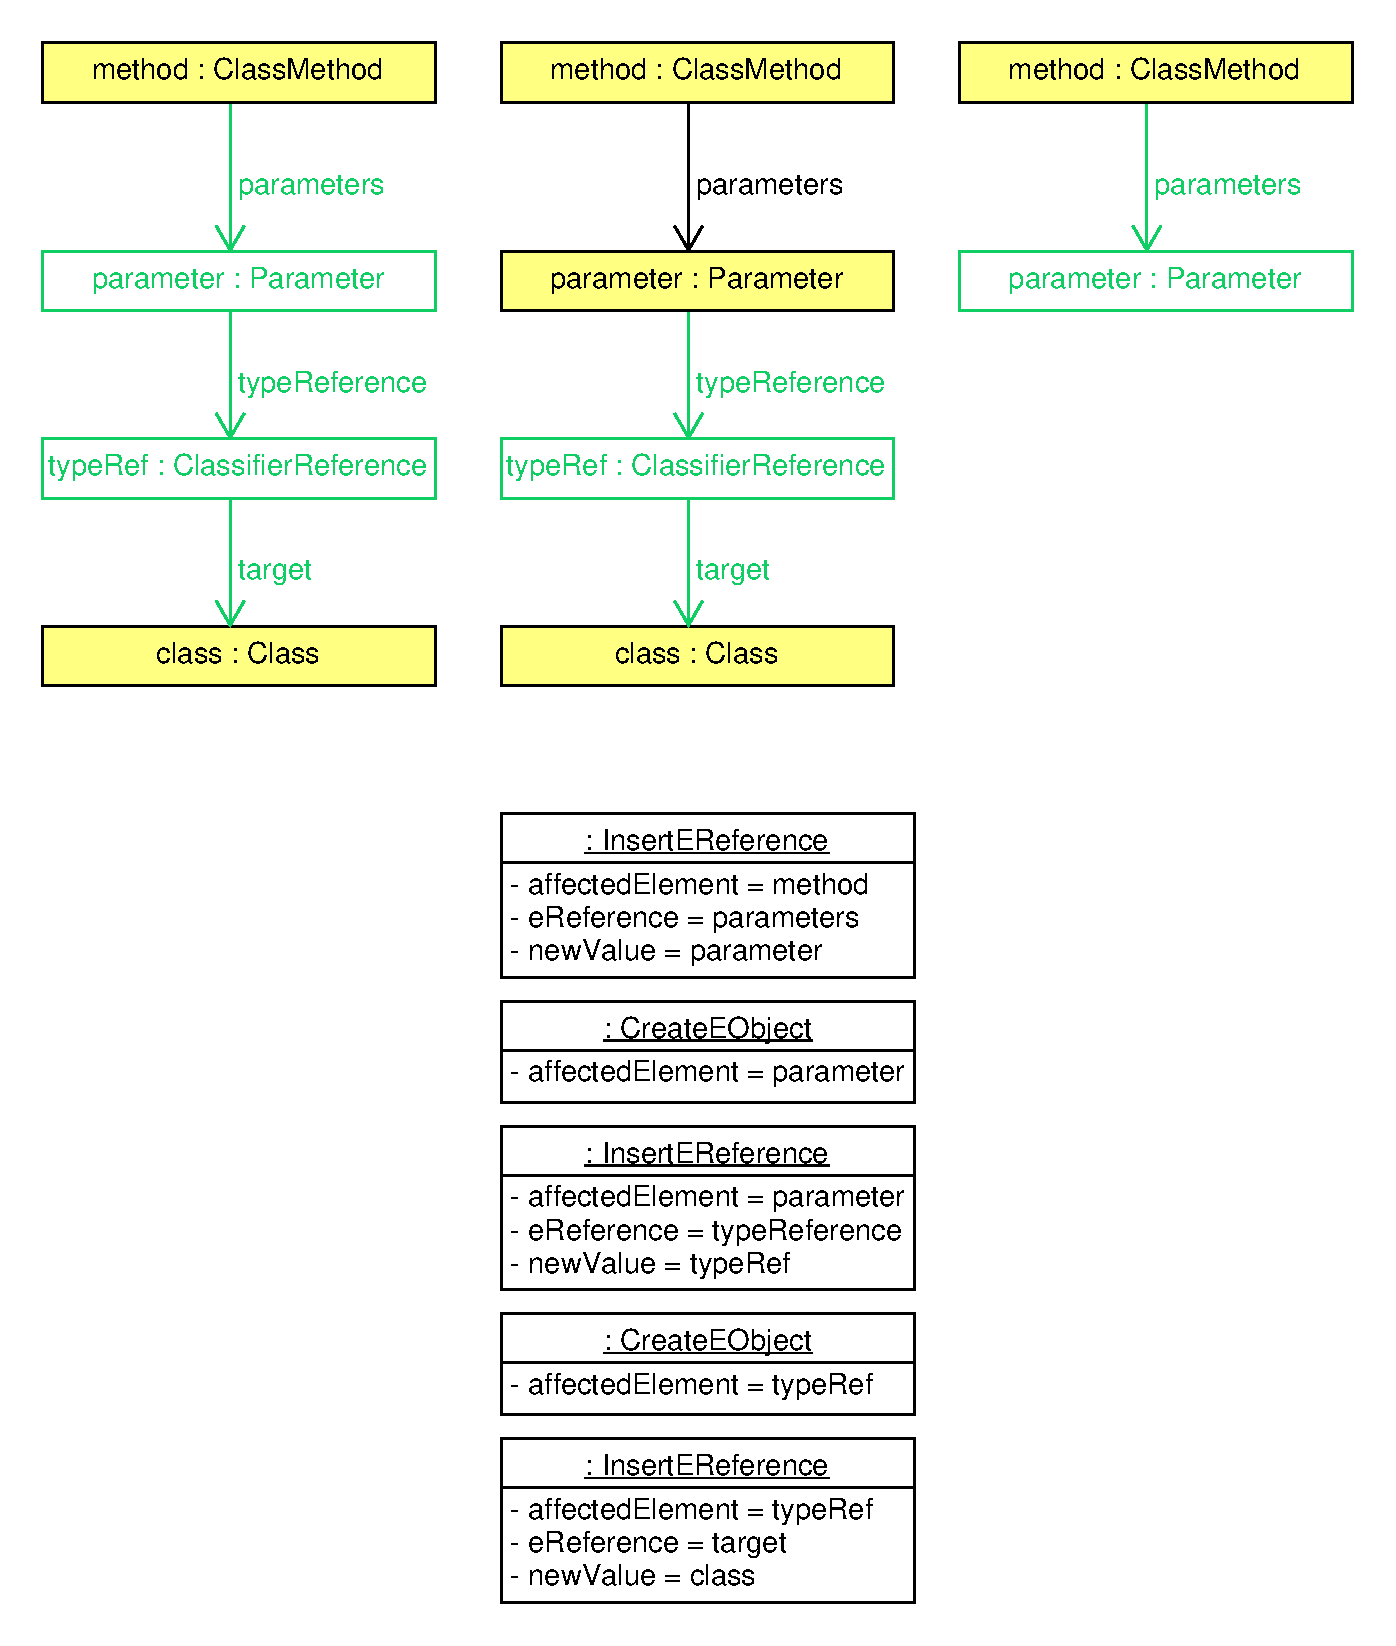
\includegraphics[width=15.8cm]{figures/tggRule_methodClassParamType_containmentExample.pdf}
\caption[Application example for the containment level heuristic]{Application example for the containment level heuristic: In the top, three source parts of TGG rules are shown. The left rule fully contains both other rules. Green matching, applied to the change sequence at the bottom of the figure, will invoke all three rules.
The dynamic containment level heuristic application algorithm will select the leftmost rule, since it contains the other two.}
\label{fig:MethodClassParamTypeContainmentExample}
\end{figure}

As envisaged by Khelladi et al. \cite{khelladi_detecting_complex_changes_2015}, this concept uses more than one heuristic at a time:
The \emph{containment level heuristic} is used first. It is modified to detect the containment level dynamically, not by pre-calculated levels, since that is not possible with a dynamic number and structure of TGG rules. In \autoref{fig:MethodClassParamTypeContainmentExample}, an application example for the containment level heuristic is shown.

Since the containment level heuristic only solves those overlap cases where one rule match completely covers another, two other heuristics are applied for the remaining conflicts. First, since it is a goal of this thesis to preserve consistency completeness, the matches with the highest coverage in the change sequence are chosen, with the intention to minimize the number of leftover EChanges that could have been matched. 
For all remaining conflicts, the \emph{distance heuristic} is used as defined by Khelladi et al. \cite{khelladi_detecting_complex_changes_2015}.

The dynamic containment level heuristic is applied as follows:
First, rule matches are sorted by the number of EChanges they cover in ascending order.
Then, for each rule match $r_i$, each rule match $r_j$ that covers more EChanges than $r_i$ is checked for containment. If $r_i$ is contained in $r_j$, $r_i$ is discarded.

% Algorithm \autoref{alg:RedMatching:DynamicContainmentLevelHeuristic} describes the application of the containment level heuristic.

% \begin{algorithm}
%     \caption{Dynamic Containment Level Heuristic}
%     \label{alg:RedMatching:DynamicContainmentLevelHeuristic}
%     \begin{algorithmic}
%         \Function{applyContainmentLevelHeuristic}{$ruleMatches$}
%             \State $sortedRuleMatches \gets \Call{sortByNumberOfEChangesAscending}{ruleMatches}$
%             \State $it \gets sortedRuleMatches.\Call{iterator}{ }$
%             \While{$it.\Call{hasNext}{ }$}
%                 \State $ruleMatch \gets it.\Call{next}{ }$
%                 \If{$it.\Call{hasNext}{ }$}
%                     % \ForAll{$containerCandidate : sortedRuleMatches.\Call{subList}{it.\Call{nextIndex}{}, n}$}
%                     \ForAll{$containerCandidate : sortedRuleMatches.\Call{subList}{it.nextIndex(), n}$}
%                         \If{$\Call{isContainedIn}{ruleMatch, containerCandidate}$}
%                             \State $ruleMatches.\Call{remove}{ruleMatch}$
%                         \EndIf
%                     \EndFor
%                 \EndIf
%             \EndWhile
%             \State \Return{$eChanges$}
%         \EndFunction
%         \newline
        
%         \Function{isContainedIn}{$potentialContainee, potentialContainer$}
%             \State $containeeEChanges \gets potentialContainee.\Call{getEChanges}{ }$
%             \State $containerEChanges \gets potentialContainer.\Call{getEChanges}{ }$
%             \State \Return{$containerEChanges.\Call{containsAll}{containeeEChanges}$}
%         \EndFunction
%     \end{algorithmic}    
% \end{algorithm}

% ---------------------------------------------------------------------------------------------------------------------------
% ---------------------------------------                RED Matching                 ---------------------------------------
% ---------------------------------------------------------------------------------------------------------------------------
\section{Red Matching: Subtractive Changes}
\label{sec:Concept:RedMatching}

In the previous sections, handling \emph{additive} EChanges that \emph{add} something to a source model and how to transport that to the target model has been covered.
However, in this concept, handling \emph{subtractive} EChanges that remove something from the model also is considered.

The \textsc{Vitruvius} change metamodel (see \autoref{sec:Foundations:Vitruvius}) also includes EChanges that are both additive and subtractive, the subclasses of \emph{ReplaceSingleValuedFeatureEChange}.
These EChanges remove the old value of an attribute or reference of an EObject and add a new value to them.
This poses a problem if one wants to map this kind of change to TGG rule applications.
In the TGG context, this change is not atomic, so this concept's approach is to split each \emph{ReplaceSingleValuedFeatureEChange} into an additive and a subtractive EChange. In the case of \emph{ReplaceSingleValuedEReference}, these are \emph{InsertEReference} and \emph{RemoveEReference}.
This split is done at the very beginning of the change propagation process, before green pattern matching.

In the following, the concept for detecting subtractive changes and repairing the TGG rule application protocol based on an atomic change sequence is described.
Without loss of generality, in this section, the assumption that the change sequence contains changes to the source model/graph is made.
Handling subtractive changes in TGGs means that we need to find out which previously applied TGG rule matches are broken because of a change to the source model.
Subsection \ref{sec:Concept:RedMatching:Implicit} and \autoref{sec:Concept:RedMatching:Explicit} describe how that detection is realizable by looking at the TGG rule application protocol and the given atomic change sequence.
Considering repair, a common strategy is to invalidate these rule applications and, cascadingly, the rule applications that have context nodes that the now-invalidated rule applications have created.
As described in \autoref{sec:Foundations:TGGs}, the concept of short-cut rules \cite{fritsche_short-cut-theoretical_2018, fritsche_short-cut-rules-repair-tgg_2021, fritsche_higher_order_short_cut_rules_2023} can be used to avoid this invalidation strategy in some cases, but not in all. Thus, the remaining cases must be dealt with.
Invalidating TGG rule applications leaves nodes and edges in the source graph uncovered by matches that potentially could be covered.
This problem is tried to be solved by re-creating EChanges from the invalidated rule applications, which is described in \autoref{sec:Concept:RedMatching:Repair}, and performing the pattern matching described in \autoref{sec:Concept:BackwardConversionPM}.

\subsection{Implicit Detection}
\label{sec:Concept:RedMatching:Implicit}
The detection of broken matches is split into implicit and explicit detection.
Implicit detection is based on the idea that each rule application recorded in the protocol that is missing a node is obviously broken.
If one assumes the change detection or recording mechanism that produces the change sequence given by \textsc{Vitruvius} is correct, this means that EChanges typed with \emph{DeleteEObject} are covered with this process.

\subsection{Explicit Detection}
\label{sec:Concept:RedMatching:Explicit}
Explicit detection means that each \emph{subtractive} EChange in the given atomic change sequence is looked upon, except \emph{DeleteEObject} and \emph{ReplaceSingleValuedFeatureEChange}. The former is covered in \autoref{sec:Concept:RedMatching:Implicit}, the latter cannot occur because, as described before, these EChanges are split up into an \emph{InsertEReference} and a \emph{RemoveEReference} EChange.

Different EChanges are handled differently; the procedure is described in the following.

\paragraph{RemoveRootEObject} This change can, but does not need to, occur together with a matching \emph{DeleteEObject} EChange, so it needs to be handled separately.
From a TGG perspective, it must have the same effects on the rule match in which the affected EObject is identified with a green node.
Thus, the rule match where the affected EObject of the RemoveRootEObject EChange occurs as bound to a green node is found and invalidated.

\paragraph{UpdateAttributeEChange}
In the case of attribute updates, it is not sufficient to only look at subtractive attribute EChanges. This is, because in some TGG formalizations, attributes are not part of the graph but of nodes of a graph. Their values are set via attribute conditions (see \autoref{sec:Foundations:eMoflon:attributeConditions}). Thus, the setting of an attribute must happen in the same rule that created its affected EObject.
That is why all \emph{UpdateAttributeEChanges}, that occur in the same atomic change sequences as the \emph{CreateEObject} EChange that has created the EObject to which the attribute belongs, are ignored in the context of detecting invalid matches.
However, those \emph{UpdateAttributeEChanges} where that isn't the case are found by searching for the rule application where the affected EObject of the \emph{UpdateAttributeEChange} is associated with a \emph{create} node. That rule application is invalidated.

\paragraph{RemoveEReference} 
A RemoveEReference EChange deletes a value out of a reference that is contained in an affected EObject. If the reference is many-valued, an index indicates the index in the EList reference.
For that kind of EChange, all TGG rule matches where the reference occurs in that constellation are found and invalidated.

\paragraph{UnsetFeature} The UnsetFeature EChange stands for unsetting the values of a feature of an affected EObject. This is handled by finding all TGG rule matches where the given feature occurs in combination with the affected EObject and invalidating them.

\subsection{Fixpoint Iterating Broken Matches}
\label{sec:Concept:RedMatching:FixpointIteration}
In \autoref{sec:Concept:RedMatching:Implicit} and \autoref{sec:Concept:RedMatching:Explicit}, the concept for determining rule applications that are invalidated by the given model change has been described.
Since there might be rule applications that use some of the \emph{create} nodes of these invalidated rule applications as \emph{context} nodes, these rule applications must also be invalidated. 
Due to the cascading nature of this invalidation, a worklist algorithm that performs fixpoint iteration on the set of invalidated rule matches has been designed (see Algorithm \autoref{alg:RedMatching:FixpointIteration}).

\begin{algorithm}
    \caption{Fixpoint Iterating Broken Matches}
    \label{alg:RedMatching:FixpointIteration}
    \begin{algorithmic}
        \Function{fixpointIterateBrokenMatches}{$brokenMatches$}
            \State $worklist \gets \Call{createNodesOf}{brokenMatches}$
            \While{$worklist \neq \emptyset$}
                \State $currentCreateNode \gets worklist.remove()$
                \State $eObject \gets \Call{getModelObject}{currentCreateNode}$
                \State $newBrokenMatches \gets \Call{intactMatchesContainingAsContext}{eObject}$
                \State $brokenMatches \gets brokenMatches$ $\cup$ $newBrokenMatches$
                \State $newCreateNodes \gets \Call{createNodesOf}{newBrokenMatches}$
                \State $worklist \gets worklist$ $\cup$ $newCreateNodes$
            \EndWhile
        \EndFunction
    \end{algorithmic}    
\end{algorithm}

\subsection{Repair}
\label{sec:Concept:RedMatching:Repair}
As matches are invalidated, model nodes become \emph{unmarked} in the sense that they are not covered by a rule application anymore.
This means that the possibility of new rule matches that cover these now unmarked nodes arises.
To account for that, this concept recreates EChanges out of those free model nodes. These EChanges form an artificial change sequence that is dealt with as a normal change sequence is, by using \autoref{sec:Concept:BackwardConversionPM:GreenMatching} and \autoref{sec:Concept:BackwardConversionPM:BlackMatching}.

For recreating EChanges out of invalidated matches, algorithm \autoref{alg:RedMatching:EChangeCreation} has been designed.
For each invalidated match, each green rule node that is still intact, meaning its mapped-to EObject has not been deleted, creates a new \emph{CreateEObject} EChange.
If the green rule has no context in the source domain, its mapped-to EObject always is a root EObject, so in that case, an \emph{InsertRootEObject} EChange is also created.
Further, for each invalidated match, all green edges that are fully intact in the model, meaning that the source and target EObject are still existing and there exists a reference from source to target that matches the green edge's type, create a new \emph{InsertEReference} EChange.

\begin{algorithm}
    \caption{Creating EChanges from Broken Matches}
    \label{alg:RedMatching:EChangeCreation}
    \begin{algorithmic}
        \Function{createEChangesForBrokenMatch}{$match$}
            % \State $worklist \gets \Call{createNodesOf}{brokenMatches}$
            % \While{$worklist \neq \emptyset$}
            %     \State $currentCreateNode \gets worklist.remove()$
            %     \State $eObject \gets \Call{getModelObject}{currentCreateNode}$
            %     \State $newBrokenMatches \gets \Call{intactMatchesContainingAsContext}{eObject}$
            %     \State $brokenMatches \gets brokenMatches$ $\cup$ $newBrokenMatches$
            %     \State $newCreateNodes \gets \Call{createNodesOf}{newBrokenMatches}$
            %     \State $worklist \gets worklist$ $\cup$ $newCreateNodes$
            % \EndWhile
            \State $eChanges \gets \emptyset$
            \ForAll{$createNode : match.getIntactCreateNodes()$}
                \State $eChanges \gets eChanges$ $\cup$ $\Call{CreateEObject}{createNode}$
                \If{$\Call{hasNoIncomingContextOrCreateEdges}{ruleNode}$}
                    \State $eChanges \gets eChanges$ $\cup$ $\Call{InsertRootEObject}{createNode}$
                \EndIf
            \EndFor
            
            \ForAll{$createEdge : match.getIntactCreateEdges()$}
                \State $eChanges \gets eChanges$ $\cup$ $\Call{InsertEreference}{createEdge}$
            \EndFor
            \State \Return{$eChanges$}
        \EndFunction
    \end{algorithmic}    
\end{algorithm}


\chapter{Implementation}
\label{ch:Implementation}

To evaluate and refine the concept and integrate it into the \textsc{Vitruvius} framework, a prototype was implemented.
The implementation uses the \emph{eMoflon::IBeX} TGG framework (\cite{eMoflonIBeX_weidmann_incremental_nodate}, see \autoref{sec:Foundations:eMoflon}), which was originally developed as a set of plugins for the \emph{Eclipse} IDE. This made the development process challenging to a certain extent.
The prototype was written in Java-21 \cite{noauthor_jdk_21nodate}.

In the following, noteworthy aspects of the prototype implementation are described.
First, in \autoref{sec:Implementation:ChangesToVitruvius}, changes that have been made to \textsc{Vitruvius} to enable propagating sequences of changes at one go are described.
Section \ref{sec:Implementation:ChangesSequenceTemplates} explains details of the realization of \emph{Change Sequence Templates}, their instantiation, matching, and initialization.
Then, in \autoref{sec:Implementation:PatternMatchingProcess} details of the pattern matching process that is prescribed by eMoflon::IBeX to a certain extent are shown.
Section \ref{sec:Implementation:EnablingAttributeConstraints} describes how using attribute constraints has been enabled, and \autoref{sec:Implementation:Challenges} concludes by describing challenges with the IBeX framework that have emerged during the implementation of the prototype.

\section{Changes to \textsc{Vitruvius}}
\label{sec:Implementation:ChangesToVitruvius}
Since the concept requires retrieving a sequence of changes upon which TGG rules are matched, \textsc{Vitruvius}, which previously only supported propagating single \texttt{EChange}s one at a time, had to be modified.
That was done by adding methods to the 
\newline\texttt{ChangePropagationSpecification} interface that the \newline\texttt{TGGChangePropagationSpecification} included in this prototype implements, and changing the propagation functionality in \texttt{ChangePropagator}, both being part of the project \emph{Vitruv-Change}.

\paragraph{ChangePropagationSpecification} In the ChangePropagationSpecification interface, the two methods seen in \autoref{implChangePropSpec} are added.
\texttt{doeshandleNonAtomicChange} is added, by default returning \texttt{false} to ensure pre-existing ChangePropagationSpecification implementations' behaviour doesn't change and \texttt{propagateNonAtomicChange} isn't called if it is not implemented.
\texttt{propagateNonAtomicChange} is added and called by \texttt{ChangePropagator} (see \autoref{implChangePropagator}), to propagate a whole change sequence that is contained in the \texttt{VitruviusChange}.

\paragraph{ChangePropagator} In \texttt{ChangePropagator}, one method is modified and two methods are created to support propagating VitruviusChanges to ChangeSequenceTemplate implementations that implement \texttt{propagateNonAtomicChange} (see \autoref{implChangePropSpec}).
\texttt{propagateChanges} now calls propagateNonAtomicChange, too, which is largely based on the existing method \texttt{propagateSingleChange}. It is modified to only concern ChangePropagationSpecifications that handle non-atomic changes.
\newline It calls \texttt{propagateNonAtomicChangeForChangePropagationSpecification} on each registered ChangePropagationSpecification, which forwards the given \texttt{VitruviusChange} to those ChangePropagationSpecifications and collects their effects on their target models.
This is the entry point to the prototype.

\begin{figure}[H]
\centering
\begin{lstlisting}[language=java, caption={Added methods in \emph{ChangePropagationSpecification.xtend}}, captionpos=b, label=implChangePropSpec]
...
def boolean doesHandleNonAtomicChanges() { false }
def void propagateNonAtomicChange(
                        VitruviusChange<EObject> change, 
                        EditableCorrespondenceModelView<Correspondence> correspondenceModel,   
                        ResourceAccess resourceAccess) {
    // noop
}
\end{lstlisting}
\end{figure}

\begin{figure}[H]
\centering
\begin{lstlisting}[language=java, caption={Excerpts of changes to methods in \emph{ChangePropagator.xtend}, enabling change sequence propagation}, captionpos=b, label=implChangePropagator]
def private propagateChanges() {
		    val result = propagateNonAtomicChange()
			result += sourceChange.transactionalChangeSequence
                    .flatMapFixed[propagateSingleChange(it)]
            ...
}

def private List<PropagatedChange> propagateNonAtomicChange() {
    ...
    val propagationResultChanges = try {
        sourceChange.affectedEObjectsMetamodelDescriptors.flatMap [
            // we only want ChangePropSpecs that handle non-atomic changes
            changePropagationProvider.getChangePropagationSpecifications(it)
                .filter[it.doesHandleNonAtomicChanges()] => [
                    forEach[it.userInteractor = outer.userInteractor]
                ]
        ].toSet.flatMapFixed [
            propagateNonAtomicChangeForChangePropagationSpecification(sourceChange, it)
        ]
    }
    ...
}

def private propagateNonAtomicChangeForChangePropagationSpecification(
    VitruviusChange<EObject> change,
    ChangePropagationSpecification propagationSpecification
) {
    val transitiveChanges = modelRepository.recordChanges [
        propagationSpecification.propagateNonAtomicChange(change, 
                modelRepository.correspondenceModel,
                modelRepository)
    ]
    // Store modification information
    changedResources += transitiveChanges.flatMap[it.affectedEObjects]
            .map[eResource]
            .filterNull
    return transitiveChanges
}
\end{lstlisting}
\end{figure}

\section{Change Sequence Templates}
\label{sec:Implementation:ChangesSequenceTemplates}
In \autoref{sec:Concept:BackwardConversionPM:BackwardConversion}, the concept and structure of \emph{Change Sequence Templates} was described. This section presents noteworthy implementation details of the prototype.

In the prototype implementation, \texttt{ChangeSequenceTemplates} and \texttt{EChangeWrappers} have different states and roles in the pattern matching process. Those are illustrated in \autoref{fig:ChangeSeqTemplateInstanceDiagramDifferentStates}. The pattern conversion step produces a \texttt{ChangeSequenceTemplateSet}. The ChangeSequenceTemplates and their EChangeWrappers contained in that ChangeSequenceTemplateSet have an implicit parent/original role. They do not and will not hold any \texttt{EObject}s, they are templates to be copied and thus instantiated.

\begin{figure}
\centering
\includegraphics[width=15.5cm]{figures/ChangeSeqTemplateInstanceDiagramDifferentStates.pdf}
\caption[Different states and roles of \texttt{ChangeSequenceTemplate}s]{Different states and roles of \texttt{ChangeSequenceTemplate}s. The originals, which serve as templates for instantiating ChangeSequenceTemplates that serve an instance role, are shown in the blue box, along with the \texttt{ChangeSequenceTemplateSet} containing them. The orange box in the bottom left shows an instantiated (note the \emph{original} references) and partly initialized ChangeSequenceTemplate, where one EChangeWrapper is partly initialized and one placeholder is fully initialized. In the green box to the bottom right, the same ChangeSequenceTemplate is shown after it has been fully matched.}
\label{fig:ChangeSeqTemplateInstanceDiagramDifferentStates}
\end{figure}

For instantiation, \texttt{getAndInitRelevantChangeSequenceTemplatesByEChange} is called on a ChangeSequenceTemplateSet, returning one or more instances of each ChangeSequenceTemplate that contains an EChangeWrapper that is matchable to an EChange. For each matchable EChangeWrapper, one instance is created and initialized with the EChange, as can be seen in \autoref{implChangeSequenceTemplateSetGetAndInit}.
To reduce both runtime and complexity, a \texttt{HashMap} that maps \texttt{EChange} \texttt{EClass}es to the Set of ChangeSequenceTemplates that contain at least one EChangeWrapper of that type is used.

The ChangeSequenceTemplate instances created by \newline\texttt{getAndInitRelevantIbexPatternTemplatesByEChange} now each have one EChangeWrapper initialized fully. Because of the placeholder structure, this might indirectly initialize other EChangeWrappers \emph{partially} or \emph{fully}.
An EChangeWrapper is fully initialized if all of its \texttt{EObjectPlaceholder}s are holding an EObject.
Thus, at this point, some of the returned ChangeSequenceTemplates are partially or fully initialized (see \autoref{implChangeSequenceTemplateSetGetAndInit}).
After pattern matching, they are either fully initialized, indicating a successful green match, or discarded.

In the following, the mechanisms of matching and initializing EChangeWrappers are described, followed by an explanation of the copy mechanism.

\begin{figure}[H]
\centering
\begin{lstlisting}[language=java, caption={Change Sequence Template Instantiation in \texttt{ChangeSequenceTemplateSet}}, captionpos=b, label=implChangeSequenceTemplateSetGetAndInit]
public Set<ChangeSequenceTemplate> getAndInitRelevantChangeSequenceTemplatesByEChange(
        EChange<EObject> eChange) {
    Set<ChangeSequenceTemplate> partlyInitializedTemplates = new HashSet<>();
    for (ChangeSequenceTemplate changeSequenceTemplate : changeSequenceTemplatesByEChangeType
            .get(eChange.eClass())) {
        changeSequenceTemplate.getEChangeWrappers().stream()
            .filter(eChangeWrapper -> eChangeWrapper.matches(eChange))
            .forEach(eChangeWrapper -> {
                ChangeSequenceTemplate changeSequenceTemplateCopy = 
                        changeSequenceTemplate.deepCopy();
                changeSequenceTemplateCopy
                    .getThisInstancesEChangeWrapperFromParent(eChangeWrapper)
                    .initialize(eChange);
                partlyInitializedTemplates.add(changeSequenceTemplateCopy);
            });
    }
    return partlyInitializedTemplates;
}
\end{lstlisting}
\end{figure}


\subsection{Matching and initialization}
\label{sec:Implementation:MatchingAndInit}
The methods for matching and initializing an EChangeWrapper form a pair. They are similarly structured and intended to be called after one another.
First, \emph{matches} is called on an EChange, checking equality of the type of the given \texttt{EChange} and the EChangeWrappers \texttt{EChange} type, and, if present, all \texttt{EObject}s contained in placeholders of the EChangeWrapper. This flexibility in matching is needed because EChangeWrappers might be partly initialized by other EChangeWrappers of the same ChangeSequenceTemplates having been initialized before and sharing placeholders.
For different kinds of \texttt{EChange}s, different subclasses of EChangeWrapper are defined. Those hold different additional fields and placeholders for further \texttt{EObject}s that an \texttt{EChange} might contain. As subclasses differ in what they hold, matching and initializing an EChangeWrapper must be subclass-specific.
To realize that, both methods follow a similar concept: The \texttt{EChange} type, meaning its EClass, and the affectedEObject are handled in the abstract \texttt{EChangeWrapper} parent class by the methods \texttt{initialize} and \texttt{matches}. The additional matching checks and initialization are handled in subclasses that implement the abstract methods \texttt{initializeExtension} and \texttt{extendedDataMatches}, as shown in \autoref{implMatchingAndInit}.

\begin{figure}[H]
\centering
\begin{lstlisting}[language=java, caption={Matching and initialization in \texttt{EChangeWrapper}}, captionpos=b, label=implMatchingAndInit]
public boolean matches(EChange<EObject> eChange) {
    return  eChangeTypeAndAffectedEObjectMatches(eChange) && extendedDataMatches(eChange);
}
public void initialize(EChange<EObject> eChange) {
    this.setEChange(eChange);
    this.getAffectedElementPlaceholder().initialize(Util.getAffectedEObjectFromEChange(eChange));
    // delegate further initialization to subclasses
    this.isInitialized = true;
}

protected abstract void initializeExtension(EChange<EObject> eChange);
protected abstract boolean extendedDataMatches(EChange<EObject> eChange);

\end{lstlisting}
\end{figure}

\subsection{Copy mechanism}
\label{sec:Implementation:CopyMechanism}
As mentioned before, ChangeSequenceTemplate \emph{parents} are created by pattern conversion (\texttt{IbexPatternToChangeSequenceTemplateConverter}) and instantiated in the process of pattern matching.
This raises the need for a copy mechanism that keeps the ChangeSequenceTemplate's EChangeWrapper and placeholder structure.
Its implementation is shown in \autoref{implCSTdeepCopy}.
First, each EChangeWrapper is copied shallowly, meaning that the placeholders in the new EChangeWrappers remain the same as in their original. The new EChangeWrapper gets a reference to its original by setting the \texttt{original} field. A mapping of old to new EChangeWrappers is created.
Then, a mapping of old to new \texttt{Placeholders} is created and handed to each EChangeWrapper to replace their old placeholders with new ones.
Finally, a new ChangeSequenceTemplate is created via a copy constructor that takes the new EChangeWrappers and the map.
The map is used by the instance to be able to retrieve EChangeWrapper instances given an \texttt{original} EChangeWrapper, as is done in \autoref{implChangeSequenceTemplateSetGetAndInit} by calling \texttt{getThisInstancesEChangeWrapperFromParent}.

\begin{figure}[H]
\centering
\begin{lstlisting}[language=java, caption={Copy mechanism in \texttt{ChangeSequenceTemplate}}, captionpos=b, label=implCSTdeepCopy]
public ChangeSequenceTemplate deepCopy() {
        Collection<EChangeWrapper> newEChangeWrappers = new LinkedList<>();
        Map<EChangeWrapper, EChangeWrapper> oldToNewEChangeWrapperMap = new HashMap<>();
        for (EChangeWrapper changeWrapper : this.eChangeWrappers) {
            EChangeWrapper newEChangeWrapper = changeWrapper.shallowCopy();
            oldToNewEChangeWrapperMap.put(changeWrapper, newEChangeWrapper);
            newEChangeWrappers.add(newEChangeWrapper);
        }
        Map<EObjectPlaceholder, EObjectPlaceholder> oldToNewPlaceholders = newEChangeWrappers
                .stream()
                .flatMap(eChangeWrapper -> eChangeWrapper.getAllPlaceholders().stream())
                .distinct()
                .collect(Collectors.toMap(
                        eObjectPlaceholder -> eObjectPlaceholder,
                        eObjectPlaceholder -> new EObjectPlaceholder(eObjectPlaceholder
                                .getTggRuleNode())
                ));
        for (EChangeWrapper eChangeWrapper : newEChangeWrappers) {
            eChangeWrapper.replaceAllPlaceholders(oldToNewPlaceholders);
        }
        return new ChangeSequenceTemplate(this.tggRule, 
                this.iBeXContextPatternMap, newEChangeWrappers, oldToNewEChangeWrapperMap);;
    }
\end{lstlisting}
\end{figure}
% \section{Pattern Conversion}

\section{Pattern Matching Process}
\label{sec:Implementation:PatternMatchingProcess}
The implementation of the pattern matching process is considerably influenced by the synchronization algorithm and architecture of \emph{eMoflon::IBeX}, which is described in \autoref{sec:Foundations:eMoflon:syncProcess}.
This section describes the side of the process that concerns the pattern matching, which is driven by being able to correctly implement the method \texttt{updateMatches)} in \texttt{VitruviusBackwardConversionTGGEngine}.
% First, in \autoref{sec:Implementation:PatternMatchingProcess:Engine}, functionings of that class, especially the method \texttt{updateMatches}, are explained.
% In further subsections, details on dependencies of that class are described.
% That includes the \texttt{VitruviusChangePatternMatcher} (see \autoref{sec:Implementation:PatternMatchingProcess:GreenMatch}) and the \texttt{VitruviusChangeBrokenMatchMatcher} (see \autoref{sec:Implementation:PatternMatchingProcess:RedMatcher}).

\subsection{VitruviusBackwardConversionTGGEngine}
\label{sec:Implementation:PatternMatchingProcess:Engine}
This section describes functionality of the class \texttt{VitruviusBackwardConversionTGGEngine} that implements the pattern matcher interface of IBeX, called \texttt{IBlackInterpreter}
and thus serves as a partner to the \texttt{SYNC}-extending class \newline\texttt{VitruviusTGGChangePropagationIbexEntrypoint}.
The interesting parts are described in the following by elucidating noteworthy methods.

\paragraph{initPatterns} Implementing the \texttt{IContextPatternInterpreter} interface of IBeX, \newline\texttt{VitruviusTGGChangePropagationIbexEntrypoint} implements the method \texttt{initPatterns}.
This method is used to initialize the pattern matchers \texttt{VitruviusChangePatternMatcher} and \texttt{VitruviusChangeBrokenMatchMatcher}. Also, pattern conversion is triggered here, using \texttt{IbexPatternToChangeSequenceTemplateConverter}.

\paragraph{updateMatches}
As described in \autoref{sec:Foundations:eMoflon:syncProcess}, in \newline\texttt{VitruviusBackwardConversionTGGEngine}, the \texttt{updateMatches} method, shown in \autoref{implUpdateMatches} is called multiple times by \texttt{VitruviusTGGChangePropagationIbexEntrypoint} which extends the IBeX class \texttt{SYNC} that, along with further parent classes, defines the synchronization algorithm of IBeX. In the following, the handle \texttt{SYNC} is used in descriptions of the process.
Between each call and the next, the triple graph might have been changed by \texttt{SYNC}. Matches might have been applied or revoked, changing the correspondence graph, the protocol, and the target model.
First, so-called \emph{consistency matches} are initialized, if not already present, by loading the \emph{protocol} that stores rule applications from previous runs and transforming them to \texttt{VitruviusConsistencyMatch}es. That is a class implementing the IBeX interface \texttt{ITGGMatch} and is used in the prototype to represent broken matches or intact matches that have been loaded from the protocol file.
For unknown reasons, this initialization is not done by IBeX itself.
To avoid recalculating matches each time updateMatches is called, \texttt{createForwardMatchesIfNotAlreadyPresent} creates green matches one time and saves the result in a class field for further calls.
However, since some of these matches might have been already applied, the remaining green matches that have not already been applied and whose green nodes are not already covered by a match having been applied prior to the current run of \texttt{updateMatches} are calculated in \texttt{getMatchesThatHaventBeenAppliedAndAreStillIntact} (see \autoref{implGetMatchesThatHaventBeenAppliedAndAreStillIntact}).
\texttt{VitruviusBackwardConversionTGGEngine} knows about matches that have been applied by implementing the IBeX interface \texttt{IbexObserver} and observing \texttt{MATCHAPPLIED} \texttt{ObservableEvent}s.
The filtered set of matches is then again thinned out twice: First, each match undergoes context matching, as described in \autoref{sec:Concept:BackwardConversionPM:BlackMatching}. Then, match selection, as described in \autoref{sec:Concept:PatternSelection} is applied, before handing the remaining matches to \texttt{SYNC}.
After having handled the additive matches, broken matches that have not been handled yet are determined using the \texttt{VitruviusChangeBrokenMatchMatcher} (see \autoref{sec:Implementation:PatternMatchingProcess:RedMatcher} and reported to \texttt{SYNC}.
Finally, in \texttt{repairUnrepairedBrokenMatches} (see \autoref{implRepairUnrepairedBrokenMatches}), broken matches newly invalidated by the \texttt{RedInterpreter} used by \texttt{SYNC} are tried to be repaired, possibly creating and applying new additive matches (see \autoref{sec:Concept:RedMatching:Repair}).

\begin{figure}[H]
\centering
\begin{lstlisting}[language=java, caption={Copy mechanism in \texttt{ChangeSequenceTemplate}}, captionpos=b, label=implUpdateMatches]
@Override
public void updateMatches() {
    initializePreexistingConsistencyMatchesIfNotAlreadyPresent();

    createForwardMatchesIfNotAlreadyPresent();
    Set<VitruviusBackwardConversionMatch> remainingMatches = 
            getMatchesThatHaventBeenAppliedAndAreStillIntact();

    matchContext_flatten_andHandToSYNC(remainingMatches);

    Set<VitruviusConsistencyMatch> brokenMatches = getBrokenMatches();
    brokenMatches.forEach(brokenMatch -> {
        this.iMatchObserver.removeMatch(brokenMatch);
    });

    // Repair matches that are broken and have not been repaired by shortcut rules
    if (ibexOptions.repair.useShortcutRules()) {
        throw new IllegalStateException("Using shortcut rules not supported yet: 
            Need to filter out repaired matches from the broken matches...");
    }
    repairUnrepairedBrokenMatches();
}
\end{lstlisting}
\end{figure}

\paragraph{getMatchesThatHaventBeenAppliedAndAreStillIntact} The method \newline\texttt{getMatchesThatHaventBeenAppliedAndAreStillIntact}, which is depicted in \autoref{implGetMatchesThatHaventBeenAppliedAndAreStillIntact}, helps ensure that matches given to \texttt{SYNC} have not been applied before and are not containing green nodes whose matched-to \texttt{EObject} is already covered by another match having been applied before.
As mentioned before, matches that have been applied are known because \texttt{VitruviusBackwardConversionTGGEngine} implements the IBeX interface \texttt{IbexObserver}. 
From these already applied matches, the \texttt{EObject}s covered by green nodes of the TGGRule belonging to the match are collected.
Then, the green matches that are to be filtered are sorted out if they were already applied or would cover one of these previously collected, already covered \texttt{EObject}s.

\begin{figure}[H]
\centering
\begin{lstlisting}[language=java, caption={Match filtering in \texttt{VitruviusBackwardConversionTGGEngine}}, captionpos=b, label=implGetMatchesThatHaventBeenAppliedAndAreStillIntact]
private Set<VitruviusBackwardConversionMatch> getMatchesThatHaventBeenAppliedAndAreStillIntact() {
        Set<EObject> createdEObjectsAlreadyCovered = this.matchesThatHaveBeenApplied.stream()
                .map(match -> (VitruviusBackwardConversionMatch) match)
                .flatMap(match -> match.getEObjectsCreatedByThisMatch().stream())
                .collect(Collectors.toSet());

        return this.matchesFound.stream()
                .filter(match -> !this.matchesThatHaveBeenApplied.contains(match))
                .filter(match -> match.getEObjectsThisMatchWouldCreate().stream()
                        .noneMatch(createdEObjectsAlreadyCovered::contains))
                .collect(Collectors.toSet());
    }
\end{lstlisting}
\end{figure}

\paragraph{repairUnrepairedBrokenMatches} The method \texttt{repairUnrepairedBrokenMatches} (see \autoref{implRepairUnrepairedBrokenMatches}) tries to repair broken matches detected by \texttt{VitruviusChangeBrokenmatchMatcher} and invalidated by \texttt{IbexRedInterpreter}.
It does so by trying to repair broken matches using the \texttt{UnrepairedBrokenMatchOldChangesRetriever} to generate a new change sequence from those green nodes and edges of the broken matches that are still mapped to \texttt{EObject}s (see \autoref{fig:impl:brokenMatches} for an example).
This new change sequence is extended by adding all \texttt{EChange} that were left unmatched by the pattern matching of the \enquote{main} change sequence, the one that had started the change propagation process, that have not already been applied. This enables matches overspanning both change sequences to be possible.
The unmatched \texttt{EChange}s from the \enquote{main} change sequence are appended at the \emph{end} of the new change sequence to not distort the application of the distance heuristic (see \autoref{sec:Concept:PatternSelection} and \autoref{sec:Foundations:ComplexChangeDetection}).
In the example in \autoref{fig:impl:brokenMatches}, the \texttt{EChange} representing the creation of Y is in the main change sequence, and all \texttt{EObject}s that are referenced by green nodes (and their references) in the bottom graph get \texttt{EChange}s created in the new change sequence.
The resulting change sequence is given to a new \texttt{VitruviusChangePatternMatcher}, which calculates new matches.
These new matches are stored globally for \texttt{updateMatches} to hand them to \texttt{SYNC}.
Finally, the new matches are context-matched, coverage-flattened, and handed to \texttt{SYNC}, in case the current call to \texttt{updateMatches} and \texttt{repairUnrepairedBrokenMatches} was the last.

\begin{figure}
\centering
\includegraphics[width=16cm]{figures/brokenMatchExample.pdf}
\caption[Broken matches example]{TGG rule matches becoming broken after X is replaced by Y. All three rule matches are broken, and nodes remaining green in the bottom graph are now \enquote{free} to be covered by another rule match.}
\label{fig:impl:brokenMatches}
\end{figure}


\begin{figure}[]
\centering
\begin{lstlisting}[language=java, caption={repair handling in \texttt{VitruviusBackwardConversionTGGEngine}}, captionpos=b, label=implRepairUnrepairedBrokenMatches]
private void repairUnrepairedBrokenMatches() {
    Set<VitruviusConsistencyMatch> unrepairedAndUntriedBrokenMatches = this.vitruviusTGGIbexRedInterpreter.getRevokedRuleMatches().stream()
            .map(match -> (VitruviusConsistencyMatch) match)
            .filter(match -> !matchesThatHaveBeenTriedToRepair.contains(match))
            .collect(Collectors.toSet());
    if (unrepairedAndUntriedBrokenMatches.isEmpty()) {
        return; // no point
    }

    List<EChange<EObject>> newChangeSequence = new UnrepairedBrokenMatchOldChangesRetriever(
            this.observedOperationalStrategy.getResourceHandler(), 
            this.ibexOptions.tgg.flattenedTGG().getRules().stream()
                    .filter(tggRule -> !tggRule.isAbstract())
                    .collect(Collectors.toSet()),
            unrepairedAndUntriedBrokenMatches, propagationDirection
            ).createNewChangeSequence();
    newChangeSequence.addAll(vitruviusChangePatternMatcher.getUnmatchedEChanges());
    VitruviusChangePatternMatcher newVitruviusChangePatternMatcher = 
        new VitruviusChangePatternMatcher(
                VitruviusChangeFactory.getInstance()
                        .createTransactionalChange(newChangeSequence),
                changeSequenceTemplateSet
    );
    Set<VitruviusBackwardConversionMatch> newMatches = 
            newVitruviusChangePatternMatcher.getAdditiveMatches(propagationDirection);
    matchesThatHaveBeenTriedToRepair.addAll(unrepairedAndUntriedBrokenMatches);
    this.matchesFound.addAll(newMatches);
    matchContext_flatten_andHandToSYNC(newMatches);
}
\end{lstlisting}
\end{figure}

\subsection{Broken matches detection}
\label{sec:Implementation:PatternMatchingProcess:RedMatcher}
The \texttt{VitruviusChangeBrokenMatchMatcher} implements what is described in \autoref{sec:Concept:RedMatching:Implicit} and \autoref{sec:Concept:RedMatching:Explicit}.
However, the prototype has one limitation to that: \texttt{EList} indices are not stored in the protocol.
This means that the detection of \textsc{RemoveEReference} is not complete, because in case an element occurs twice in the list, the rule application match where that list insertion was marked with create nodes and edges is ambiguous.
Because of that, removing elements in lists that occur there more than once is not supported by the prototype.

\section{Enabling Attribute Constraints}
\label{sec:Implementation:EnablingAttributeConstraints}
As described in \autoref{sec:Foundations:eMoflon:attributeConditions}, eMoflon::IBeX supports defining attribute constraints to specify relationships between attributes of corresponding \texttt{EObject}s.
Because IBeX isn't designed as a library but as an Eclipse plugin, this was realized via class loading and the \emph{Java Reflection API}, which is shown in \autoref{implEnablingAttributeConstraints}.
The user must have defined custom attribute constraints in the default factory for that, which is \newline\texttt{UserDefinedRuntimeTGGAttrConstraintFactory}. That Class, although auto-generated in the process of an eMoflon build, always is contained in the same package, namely\newline
\texttt{org.emoflon.ibex.tgg.operational.csp.constraints.factories.<<projectName>>}. \newline
It is loaded and then instantiated and handed to IBeX.


\begin{figure}
    \centering
    \begin{lstlisting}[language=java, caption={Enabling Attribute Constraints in \texttt{VitruviusTGGChangePropagationRegistrationHelper}}, captionpos=b, label=implEnablingAttributeConstraints]
    private void tryToFindAndAddUserDefinedAttributeConstraints(IbexOptions ibexOptions) {
        try {
            //class loader should have access to this CL's classes as well as the ibex project
            Class userDefinedConstraintFactoryClass = new SimpleNameSupportingURLClassLoader(
                    new URL[]{new File(ibexProjectPath, "/bin").toURI().toURL()},
                    this.getClass().getClassLoader())
                    .loadClass("org.emoflon.ibex.tgg.operational.csp.constraints.factories." 
                            + ibexOptions.project.name().toLowerCase() 
                            + ".UserDefinedRuntimeTGGAttrConstraintFactory");
            ibexOptions.csp.userDefinedConstraints((RuntimeTGGAttrConstraintFactory)    
                    userDefinedConstraintFactoryClass.getConstructor().newInstance());
        } catch (MalformedURLException | InvocationTargetException | InstantiationException | 
                IllegalAccessException | NoSuchMethodException e) {
            logger.warn("Couldn't load UserDefinedRuntimeTGGAttrConstraintFactory");
        }
    }
    \end{lstlisting}
\end{figure}


\section{Challenges with the IBeX Framework}
\label{sec:Implementation:Challenges}

During the implementation of the prototype in eMoflon, a number of issues with the IBeX framework occurred, some of which could be dealt with, while others could not.
Especially the proxy issue, which had an impact on the evaluation results (see \autoref{sec:Evaluation:Results:G1}), artificially restricts the capabilities of the prototype, preventing rule applications that otherwise would be functioning.

\subsection{Solved Issues}
\label{sec:Implementation:Challenges:solved}

Some issues with the IBeX framework could be solved by overriding classes and methods from the framework. Some of these issues are bugs, others are a lacking of access to data required by the prototype implementation.
\paragraph{SmartEMF} On their website, the eMoflon developers describe \emph{SmartEMF} as a \enquote{High-performance EMF reimplementation complying with EMF interfaces} \cite{noauthor_emoflonibex_nodate}.
However, parts of the implementation do not comply with the EMF interfaces, which produced problems while testing the prototype.
One of those is \texttt{org.emoflon.smartemf.persistence.AdapterList}.

\paragraph{org.emoflon.smartemf.persistence.AdapterList} is a SmartEMF implementation of an EMF \texttt{EList<Adapter>}.
Because its internal representation is a \texttt{LinkedHashSet}, which doesnt implement \texttt{List} functions, methods like \texttt{get(int index)}, \texttt{add(int index, Adapter element)} or \texttt{indexOf(Object o)}, which have to be implemented to comply with the \texttt{EList} interface, miss data to return something meaningful. Thus, the developers of SmartEMF chose to throw an \texttt{UnsupportedOperationException} wherever these methods are called.
In preparing the evaluation, such a call occurred while loading model elements.
This issue was fixed in the \texttt{tools.vitruv.dsls.tgg.emoflonintegration.ibex.smartEmfFix} package by extending \texttt{AdapterList} with the \texttt{AdapterListFixed} class, overriding the aforementioned \texttt{indexOf} and \texttt{add} methods. \texttt{indexOf} always returns $0$, and \texttt{add} is implemented as a noop. This fixed the problem but should be kept in mind in case any persistence issue arises.
The \texttt{AdapterListFixed} was \enquote{injected} by also overriding the \texttt{SmartEMFResource} and the \texttt{SmartEMFResourceFactoryImpl} classes and registering the latter as the default \texttt{ResourceFactory} for the resourceSet of \texttt{VitruviusBackwardConversionTGGEngine}.

\paragraph{org.emoflon.ibex.tgg.operational.repair.strategies.AttributeRepairStrategy} is an IBeX class that enforces attribute constraints on matches. However, it also tries to enforce these on matches that are not fully matched, meaning that some nodes are not mapped to \texttt{EObject}s, which then results in a \texttt{NullPointerException}.
This has been fixed by extending the \texttt{AttributeRepairStrategy} with \texttt{FixedAttributeRepairStrategy} in the \newline
\texttt{tools.vitruv.dsls.tgg.emoflonintegration.ibex} package. There, the \texttt{repair} method was overridden and a \texttt{null} check added.
Similar to the \texttt{AdapterList} issue, the \newline\texttt{FlexibleSeqRepair} class, extending 
\newline\texttt{org.emoflon.ibex.tgg.operational.repair.SeqRepair}, was created to inject the \newline\texttt{FixedAttributeRepairStrategy}.

\paragraph{paranoid modifications} In the \texttt{VitruviusBackwardConversionTGGEngine}, which implements the \texttt{IBlackInterpreter} interface, the 
\texttt{getProperties} method can be overridden to, among others, set the \texttt{needs\_paranoid\_modifications} property.
While conducting the evaluation, it turned out that both states are needed.
For deleting changes, \newline
\texttt{needs\_paranoid\_modifications} being set to false leads to an \newline
\texttt{UnsupportedOperationException} being thrown in the UML EMF implementation. \newline
For additive changes, \texttt{needs\_paranoid\_modifications} being set to true makes the serialization faulty, losing some references that look like they are serialized but aren't deserialized.
This issue was again fixed by setting \texttt{needs\_paranoid\_modifications} to \texttt{false} by default and extending an IBeX class, in this case \texttt{IbexRedInterpreter}. The extending class, \texttt{VitruviusTGGIbexRedInterpreter}, overrides the \texttt{revoke(\dots)} method where it sets \texttt{needs\_paranoid\_modifications} temporarily to \texttt{true}, as can be seen in \autoref{implNeedsParanoidMod}.

\begin{figure}[H]
\centering
\begin{lstlisting}[language=java, caption={Source Model Serialization}, captionpos=b, label=implNeedsParanoidMod]
@Override
public void revoke(Set<EObject> nodesToRevoke, Set<EMFEdge> edgesToRevoke) {
    patternMatcher.setNeeds_paranoid_modificiations(true);
    super.revoke(nodesToRevoke, edgesToRevoke);
    patternMatcher.setNeeds_paranoid_modificiations(false);
}
\end{lstlisting}   
\end{figure}

\subsection{Unsolved Issues}
\label{sec:Implementation:Challenges:unsolved}
Unfortunately, some issues with eMoflon::IBeX could not be solved. As mentioned before, this distorts the evaluation results, which is also discussed in the evaluation chapter (\autoref{ch:Evaluation}).
In the following, these issues are described, as well as the reasons why they could not be solved.

\paragraph{Unresolved proxies} The proxy problem appeared in the process of the evaluation.
Some \texttt{TGGRules} contained nodes and/or references whose \texttt{type} attribute, which references the \texttt{EClass} or \texttt{EReference} that a node or an edge represents, was a \emph{proxy} (see \autoref{sec:Foundations:MDSE}), indicating that this metamodel element could not be loaded or has been unloaded.
These rules could be translated to \texttt{ChangeSequenceTemplates} by the prototype but not be matched to a \texttt{VitruviusChange}, because the proxy \texttt{EClass}es and \texttt{EReference}s could not be matched successfully to the \texttt{EObject}s' \texttt{EClass}es and the \texttt{EReference}s held by the \texttt{EChange}s.
They, however, were no proxies, which indicates that the problem does not lie with the model or its serialization being faulty but rather with the IBeX framework. 
All attempts to solve this problem failed, and since at the present time development of the IBeX framework is discontinued, a solution is likely only to be found by either forking the framework or moving to another, e.g., \emph{eMoflon::neo} \cite{weidmann_emoflonneo_nodate}.

\paragraph{Correspondence Model Serialization} Another issue that also occurred while conducting the evaluation concerned IBeX's serialization of the correspondence model.
This issue is illustrated with an example, as can be seen in \autoref{implSrcModelSerialization} and \autoref{implCorrGraphSerialization}.
In a situation where a many-valued reference has two or more values, a deletion of any but the last value results in the correspondence model serialization being corrupted. That is because, as can be seen in \autoref{implCorrGraphSerialization}, correspondence entries reference source and target entries by pointing at indexes in the respective model serialization files.
Deleting the first \texttt{members} entry named \enquote{constructer} in \autoref{implSrcModelSerialization} leads to the \texttt{source} entry in \autoref{implCorrGraphSerialization} now pointing to the formerly second, but now first \texttt{members} entry in \autoref{implSrcModelSerialization}, that is called \enquote{methed}.
In this case, IBeX won't even load the correspondence model, because the type checking of \texttt{JavaConstructorToOperation} fails, since it expects a \texttt{Constructor} as source but gets a \texttt{ClassMethod}.
If the first member were also a member, this corruption would be silent.
Like with the unresolved proxies problem, this might be solved by using another framework or implementing an alternative serialization solution that does not relate objects by position but, e.g., by ID.

\begin{figure}[H]
\centering
\begin{lstlisting}[language=xml, caption={Source Model Serialization}, captionpos=b, label=implSrcModelSerialization]
 <classifiers xsi:type="classifiers:Class" name="kless">
     <members xsi:type="members:Constructor" name="constructer">
        <parameters xsi:type="parameters:OrdinaryParameter" name="parrametr"/>
     </members>
     <members xsi:type="members:ClassMethod" name="methed">
        <parameters xsi:type="parameters:OrdinaryParameter"/>
     </members>
     <members xsi:type="members:Field" name="myField"/>
 </classifiers>
\end{lstlisting}     
\end{figure}

\begin{figure}[H]
\centering
\begin{lstlisting}[language=xml, caption={Correspondence Model Serialization},captionpos=b, label=implCorrGraphSerialization]
 <Java2Uml:JavaConstructorToOperation>
     <target xsi:type="uml:Operation" href="uml_instance.model#/0/@packagedElement.0/@ownedOperation.0"/>
     <source xsi:type="members:Constructor" href="java_instance.model#//@compilationUnits.0/@classifiers.0/@members.0"/>
 </Java2Uml:JavaConstructorToOperation>
\end{lstlisting}       
\end{figure} 

%% LaTeX2e class for student theses
%% sections/evaluation.tex
%% 
%% Karlsruhe Institute of Technology
%% Institute of Information Security and Dependability
%% Software Design and Quality (SDQ)
%%
%% Dr.-Ing. Erik Burger
%% burger@kit.edu
%%
%% Version 1.6, 2024-06-07

\chapter{Evaluation}
\label{ch:Evaluation}
The purpose of the evaluation of the implemented prototype is to empirically assess the capabilities of the developed approach to pattern matching of TGG rules on atomic model changes.

Therefore, one concern is to determine the automatization degree in terms of consistency completeness, i.e., the expressiveness for consistency conditions, the rule representation complexity (the avoidance of data loss) and performance of TGG usage on available \textsc{Vitruvius} evaluation cases like those used in the article describing the \textsc{Vitruvius} approach \cite{VitruviusKlare2021} and based on that compare them with preexisting consistency preservation languages.
To that end, the evaluation cases were extended, translating existing rules to TGG rules wherever possible.

A second concern, that of scalability, was evaluated by randomly generating models from the TGG rules in the evaluation case \emph{HospitalToAdministration}, which is from the emoflon::IBeX tutorial \cite{emoflon_tutorial, noauthor_github_emoflon_tutorial}.
The idea is to generate models of various sizes and measure the asymptotical runtime performance of the prototype.

\section{GQM Plan}
\label{sec:Evaluation:GQMPlan}
The evaluation is structured by following a Goal Question Metric (GQM) plan, as proposed by Basili et al. \cite{basili_methodology_gqm_1984}, to enable transparent methodical verifiability and to explicitly consider construct validity.

\begin{gqm}
    \item Ensuring correctness of the consistency preservation process
    \begin{gqm}
        \item Does the approach identify complex changes correctly?
        \begin{gqm}
            \item Number of change sequences that are incorrectly matched
        \end{gqm}
    \end{gqm}
    \item Preserving consistency completeness
    \begin{gqm}
        \item Can realistic consistency relations be represented by the TGG approach?
        \begin{gqm}
            \item Number of rules that can be represented by TGG rules.
        \end{gqm}
    \end{gqm}
    \item Preserving or improving performance of consistency preservation
    \begin{gqm}
        % \item How does the TGG approach perform in comparison to existing approaches in (semi-) realistic scenarios
        % \begin{gqm}
        %     \item Runtime of consistency preservation algorithm on change sequences
        % \end{gqm}
        \item How does the approach perform in comparison to existing approaches?
        \begin{gqm}
            \item Runtime trend of consistency preservation algorithm on change sequences in dependence of input nodes and change sequence length.
            \item Runtime trend of different subroutines of the consistency preservation algorithm on change sequences in dependence of input nodes and change sequence length.
        \end{gqm}
    \end{gqm}
\end{gqm}

In \autoref{sec:Evaluation:Design}, the realization of the GQM plan are explained in full detail.
Section \ref{sec:Evaluation:Results} presents and discusses the results of the evaluation according to the method described in \autoref{sec:Evaluation:Design}.

\section{Method}
\label{sec:Evaluation:Design}
In this section, the general preconditions for conducting the evaluation are described. This includes the used evaluation cases and the procedure.
Then, each goal described in the GQM Plan (see \autoref{sec:Evaluation:GQMPlan}) and their respective setup constellations are explained.

\paragraph{Evaluation Cases} In the preparation of this evaluation, two evaluation cases were chosen for the accomplishment of the three goals to depend on:
\begin{itemize}
    \item \textbf{G1}, \textbf{G2}: \emph{JavaToUml} \cite{noauthor_vitruv-toolsvitruv-casestudies_nodate, chen_java-to-uml} 
    \item \textbf{G3}: \emph{HospitalToAdministration} \cite{emoflon_tutorial, noauthor_github_emoflon_tutorial}
\end{itemize}

In the case of \emph{JavaToUml}, existing consistency preservation rules, written in the reactions language \cite{kramer_specification_2017}, were attempted to translate into TGG rules by hand.
% \todo{JavaToUml detaillierter beschreiben, Metamodelle und bestehende reactions}

\subsection{G1 - Ensuring correctness of the consistency preservation process}
\label{sec:Evaluation:Design:G1}
Ensuring correctness of the consistency preservation process is the first goal of the evaluation of the prototype.
The TGG rules written for the two evaluation cases form the basis for being able to reach that goal.
The following question is answered:

\paragraph{Q1.1} Does the approach identify complex changes correctly?\newline
To answer that question, we define a number of change sequences so that each TGG rule is covered at least once.
We further define which matches are expected for each change sequence.
Based on that, the number of change sequences whose matches deviates from the expectation, and are thus \emph{incorrectly matched}, is determined.
Further, that same number of incorrectly matched patterns under the fiction of not having the proxy problem described in \autoref{sec:Implementation:Challenges:unsolved} is determined. Due to the fictional nature, this is done by comparing the change sequences that are incorrectly matched due to the proxy problem to other change sequences that don't fall under the proxy problem and assuming that they would behave in the same way. For each of those, a \enquote{partner rule} is determined to make this metric more traceable and replicable.

Since the outcome of that metric and its proxy-problem ignoring counterpart depends on how change sequences are chosen, their choice is oriented towards the evaluation case.

% This way, the first metric indicates how often incorrectly matched patterns occur and the second metric indicates how many rules can be expected to be \enquote{safe to use}.


\subsection{G2 - Preserving consistency completeness}
\label{sec:Evaluation:Design:G2}
To evaluate to what extend the goal of preserving consistency completeness is reached, the following question is answered:

\paragraph{Q2.1} Can realistic consistency relations be represented by the TGG approach? \newline
The choice of using the evaluation case \emph{JavaToUml} for the evaluation roots in this question. Both Java and UML are non-artificial metamodels which have been modeled in the Eclipse Modeling Framewok. Since there are overlaps in the concepts that both metamodels describe, consistency relations between both metamodels can be deemed realistic and have also been modeled in the \emph{Reactions} language \cite{kramer_specification_2017} prior to this thesis.
To answer the question, that \emph{consistency preservation rules} (CPRs), represented by reactions, are looked upon. 
The effects of each reaction are tried to be modeled with TGG rules that are processable in the prototype.
Then, each rule is categorized into one of the following categories:
\begin{itemize}
    \item \emph{Full preservation}: The consistency preservation rule is equivalently implemented by both the reaction and the TGG rule(s).
    \item \emph{Partial preservation}: The consistency preservation rule expressed by the reaction can only be implemented partially by TGG rules. Some aspects are implementable and processable, some are not.
    \item \emph{No preservation} The consistency preservation rule can not be expressed with TGG rules or not be processed by the prototype
\end{itemize}
For each category, the number of CPRs that fall into that category is determined. For partial or no preservation, reasons are given.


\subsection{G3 - Preserving or improving performance of consistency preservation}
\label{sec:Evaluation:Design:G3}
Having set the goal of preserving or improving performance of consistency preservation with the concept, the following question is to be answered:

\paragraph{Q3.1} How does the approach perform in comparison to existing approaches? \newline
The question of performance and scalability rises as using preexistent information on the actual changes to generate matches is an approach in which the search space is smaller and thus, it can be hypothesized that less computing time is needed to find rule matches and propagate them to the target model.
However, since the concept and prototype include a selection of pattern matches (see \autoref{sec:Concept:PatternSelection}), this must be taken into account when comparing the approach to another pattern matcher that does not perform this.
The other pattern matcher is the \emph{high-performance pattern matcher} \textsc{HiPE} \cite{hipe-devops_highly_2022} included in the eMoflon::IBeX framework.
For easier referencing, the approach in this thesis is called \textsc{VitruvTGG} in the context of evaluation.
The following time measurements are taken:
\begin{itemize}
    \item \textsc{VitruvTGG}: 
        \begin{itemize}
            \item Main green forward matching time: The time spent for the green matching of the change sequence against the ChangeSequenceTemplates
            \item Total context matching time: The cumulated time spent on trying to match context for green matches that have not yet been applied.
            \item Total coverage flattening time: The cumulated time spent on \emph{coverage flattening}, i.e. ensuring that each change is covered by at most one match.
            \item Total change propagation time: The total runtime of the change propagation
        \end{itemize}
    \item \textsc{HiPE}: Total change propagation time: The total runtime of the change propagation
\end{itemize}

\paragraph{Experimental Setup}
The experimental setup is designed in the following way:
Models, and thus change sequences, of different sizes are generated randomly with the eMoflon::IBeX \textsc{Modelgen} application. This application generates a \enquote{random} triple graph based on a TGG ruleset. \textsc{Modelgen} has limitations that restrict the choice of model size measure. While it is possible to specify a maximum amount of graph elements this cannot be the only constraint since \textsc{Modelgen} only applies one rule if only that constraint is given. To nudge \textsc{Modelgen} to more randomness, the max count of rules is also included, calculated as follows: $maxApplicationsPerRule=graphElementSize / numberOfRules$.
Although a rule application always creates at least one graph element, These further constraints have repercussions on the resulting graph element size, because situations might occur where some rules have reached their max count and all others are not applicable to the current situation anymore.
The procedure is as follows: For $graphElementSize = 2^3, 2^4, \dots, 2^{11}$, the following steps are taken with both the \textsc{HiPE} and the \textsc{VitruvTGG} pattern matcher:
\begin{enumerate}
    \item Generate triple graph with source element size $graphElementSize$ and the aforementioned additional constraints.
    \item Delete correspondences, protocol and target graph.
    \item Generate a change sequence from $\emptyset$ to $model$ using \textsc{Vitruvius} classes that use EMF Compare \cite{noauthor_emf_compare}.
    \item Start change propagation and measure the times described above.
    \item Repeat steps 1 to 4 with this parametrization $20$ times.
    \item calculate the median and store the results.
\end{enumerate}
That procedure is automated using \emph{JUnit 5} \cite{noauthor_junit_nodate}.
Performance measurements are executed on a machine with the following specifications:
\begin{itemize}
    \item Processor: Intel Core i9-8950HK
    \item Random Access Memory: $32.0$ GB, $2667$ MHz
    \item Operating System: Windows 10 Pro
\end{itemize}


% \paragraph{Q3.2} \todo{TODO EVENTUELL}: Check second approach: generate 2048-model and don't delete corr, source and target! Perform 8,16,32,64,128,256,512,... changes. Hypothesis: Here, Vitruv might perform bettern than in Q3.1 since the prototype  knows where the changes happened.
% The question of performance and scalability rises as using preexistent information on the actual changes to generate matches is an approach in which the search space is smaller
% \todo{schreibne}

\section{Results}
\label{sec:Evaluation:Results}
In this section, the results of the evaluation that was performed following the method in \autoref{sec:Evaluation:Design} are presented.

\subsection{G1 - Ensuring correctness of the consistency preservation process}
\label{sec:Evaluation:Results:G1}
In \autoref{tab:M1.1.1}, the results of evaluating the prototype on \emph{JavaToUML} with metric \emph{M1.1.1} can be seen.
It is noticeable, that while with $57.78\%$, the number of correctly matched patterns can be considerd relatively low, the number of correctly matched patterns if there was no proxy problem is relatively high ($95.56\%$).
That can be interpreted as a good sign for the correctness of the concept but a drawback for the prototype or the framework that introduces the proxy problem. 
\begin{table}[h!]
\centering
\begin{tabular}{c | c  c c c}
    \toprule
     &      & \multicolumn{3}{c}{matching categories} \\
            & total & \makecell{incorrectly \\ matched} & \makecell{correctly \\ matched} & \makecell{correctly matched \\ if there was no proxy problem}\\
    \midrule
    \makecell{Number of \\ change sequences}  & $45$ & $19$ & $26$ & $43$\\
    Proportion of total    & $100\%$ & $42.22\%$ & $57.78\%$ & $95.56\%$ \\
    % 789 & 0AB\\
    \bottomrule
\end{tabular}
\caption{Results of metric M1.1.1 on evaluation case JavaToUml}
\label{tab:M1.1.1}
\end{table}

\subsection{G2 - Preserving consistency completeness}
\label{sec:Evaluation:Results:G2}
In \autoref{tab:M2.1.1}, the results of evaluating the prototype on \emph{JavaToUML} with metric \emph{M2.1.1} can be seen.
With  $93.33\%$, consistency completeness can be interpreted as high, considering that the baseline is a turing-complete imperative language while the protoype's imperativity is limited to attribute conditions.

\begin{table}[h!]
% \centering\small
\centering
\begin{tabular}{c | c  c c c}
    \toprule
     &      & \multicolumn{3}{c}{representability} \\
            & total & full & partial & None \\
    \midrule
    Number of consistency preservation rules  & $45$ & $42$ & $2$ & $1$\\
    Proportion of total    & $100\%$ & $93.33\%$ & $4.44\%$ & $2.22\%$ \\
    % 789 & 0AB\\
    \bottomrule
\end{tabular}
\caption{Results of metric M2.1.1 on evaluation case JavaToUml}
\label{tab:M2.1.1}
\end{table}

The cases where the consistency preservation rules defined in the \emph{Reactions} langugage could not be fully represented and the reasons for that are discussed in the following.

Reactions that could only be partially reppresented with TGG rules include \newline\texttt{JavaCompilationUnitInsertedInPackage} and \texttt{JavaClassifierRemoved}.
\newline\texttt{JavaCompilationUnitInsertedInPackage}, as can be seen in \autoref{javaCompilationUnitInsertedInPackage} includes adding correspondences between the metamodel element \texttt{UMLPackage.Literals.PRIMITIVE\_TYPE} and model elements. This cannot be mapped with TGGs.


\begin{figure}
\centering
\begin{lstlisting}[language=java, caption={Reaction JavaCompilationUnitInsertedInPackage},captionpos=b, label=javaCompilationUnitInsertedInPackage]
reaction JavaCompilationUnitInsertedInPackage {
	after element java::CompilationUnit inserted in java::Package[compilationUnits]
	call {
		rootElementPreSetup(newValue)
		newValue.classifiers.forEach[insertUmlClassifierIntoPackage(it, affectedEObject)]
	}
}
routine rootElementPreSetup(EObject alreadyPersistedEObject) {
	update {
		detectOrCreateUmlModel(alreadyPersistedEObject)
		registerPredefinedUmlPrimitiveTypes(alreadyPersistedEObject)
	}
}
routine registerPredefinedUmlPrimitiveTypes(EObject alreadyPersistedEObject) {
	update {
		getNotRegisteredPrimitiveTypesWithUnifiedNames([ sourceElement, expectedType, tag |
			getCorrespondingElement(sourceElement, expectedType, null, tag, false)
		], alreadyPersistedEObject.eResource.resourceSet).forEach [
			addCorrespondenceBetween(UMLPackage.Literals.PRIMITIVE_TYPE, it.key, it.value)
		]
	}
}
\end{lstlisting}  
\end{figure}

The reaction JavaClassifierRemoved could only be represented partly, because in the TGG implementation used in the approach, deleting a model element always means invalidating the rule that has created it.
In JavaClassifierRemoved, as can be seen in \autoref{javaClassifierRemoved}, if a $Classifier$ is removed, the $CompilationUnit$ it belongs to is automatically removed, too. However, this relation is not symmetric in a sense that $Classifier$ and $CompilationUnit$ are always required to be created together, since two reactions are responsible for that, \texttt{JavaCompilationUnitInsertedInPackage} and \texttt{JavaClassifierInserted}.
Representing this in TGGs either means representing these two reactions with one TGG rule for each reaction, as can be seen in \autoref{fig:classToUmlClass}, or representing both reaction with a single TGG rule.
In the former case, the option to create a $Classifier$ independent of its $CompilationUnit$ gets lost, thus those two would only be partly represented. In the latter case, which is the one that was chosen, \texttt{JavaClassifierRemoved} is only represented partly, as only the $Classifier$ would be removed by revoking the respective additive rule, and the $CompilationUnit$ would survive.

\begin{figure}
\centering
\begin{lstlisting}[language=java, caption={Reaction JavaCompilationUnitInsertedInPackage},captionpos=b, label=javaClassifierRemoved]
reaction JavaClassifierRemoved {
	after element java::ConcreteClassifier removed from java::CompilationUnit[classifiers]
	call cleanUpJavaCompilationUnit(affectedEObject)
}
routine cleanUpJavaCompilationUnit(java::CompilationUnit jCompUnit) {
	update {
		removeObject(jCompUnit)
	}
}
\end{lstlisting}  
\end{figure}

\begin{figure}
\centering
\includegraphics[width=15.5cm]{figures/tggRule_classToUmlClass.pdf}
\caption{TGG rule ClassToUmlClass}
\label{fig:classToUmlClass}
\end{figure}


\subsection{G3 - Preserving or improving performance of consistency preservation}
\label{sec:Evaluation:Results:G3}
In \autoref{fig:eval:RuntimeTrend}, the results of evaluating the prototype on \emph{HospitalToAdministration}, a case from the emoflon::IBeX tutorial \cite{emoflon_tutorial, noauthor_github_emoflon_tutorial}, using metric \emph{M3.1.1} can be seen. \textsc{VitruvTGG} performs slightly better or equal to \textsc{HiPE} up to a model size of 128 model elements (\textsc{VitruvTGG}: 116ms, \textsc{HiPE}: 115ms). From there on, \textsc{VitruvTGG} performance diverges strongly from \textsc{HiPE}'s performance.
To find out the reason for that, sub-measurements are included in \autoref{fig:eval:RuntimeTrend}. Looking at these, it stands out that coverage flattening takes up most of the total time of \textsc{VitruvTGG}, from $216$  model elements upwards it even surpasses the total execution time of \textsc{HiPE}, while the more matching-relevant measurements \emph{main green matching} and \emph{context matching} stay faster than \textsc{HiPE}, although from $4096$ model elements upwards, in tha case of \emph{main green matching}, that can be expected to change as well, but not drastically, regarding the course of the curves.
Since \emph{coverage flattening}, while being useful to find the \emph{intended} rule matches (as discussed in \cite{khelladi_detecting_complex_changes_2015}), is not necessary for the \emph{correctness} of the matching, it is of interest to look at the performance of \textsc{VitruvTGG} if coverage flattening is omitted. That is simulated by subtracting the coverage flattening time from the total change propagation time and shown in \autoref{fig:eval:RuntimeTrendWithoutCoverageFlattening}.
There it can be seen what has been suspected: While \textsc{VitruvTGG} performs better until a model size of $256$ or $512$ elements, performance diverges from there on upwards, although not as steeply as before.

To summarize, it can be said that \textbf{Q3.1} has to be answered in a differentiated way: In comparison to \textsc{HiPE}, the approach performs better or equally up to a problem size of $128$ and worse from there on upwards. So, whether \textbf{G3} has been reached depends on what problem sizes are regarded: Performance is improved or preserved and \textbf{G3} is reached for problem sizes smaller as $128$ changes in a sequence, for larger sequences, it is not and \textbf{G3} is not reached.

\begin{figure}[h!]
    \centering
    \begin{tikzpicture}
        \definecolor{myBlue}{RGB}{33,92,255}
        \definecolor{myRed}{RGB}{255,43,54}
        \definecolor{myGreen}{RGB}{42,174,105}
        \definecolor{myPurple}{RGB}{174,42,110}
        \begin{axis}[
            width=0.9\textwidth,
            height=0.9\textwidth,
            xlabel={Number of model elements in the Change Sequence},
            ylabel={Time [ms]},
            xmin=0, xmax=4096,
            ymin=0, ymax=1400000,
            xticklabels={4,8,16,32,64,128,256,512,1024,2048,4096},
            % ytick={0,10,100,1000,10000,100000},
            legend pos=north west,
            ymajorgrids=true,
            grid style=dashed,
            xmode=log,
            ymode=log,
            log basis x={2},
            log basis y={2}
        ]
        
        % VitruvTGG main green matching:
        \addplot[
            color=myGreen,
            mark=triangle,
            smooth,
            opacity=0.4,
            ]
            coordinates {
            % (8,0)(16,6)(32,4)(64,9)(128,12)(256,45)(512,145)(1024,564)(2048,2191)
            (8,0)(16,6)(32,6)(64,17)(128,14)(256,49)(512,168)(1024,823)(2048,2308)(4096,8982)
            };
        % % VitruvTGG context matching:
        \addplot[
            color=black,
            mark=triangle,
            smooth,
            opacity=0.4,
            ]
            coordinates {
            % (8,0)(16,3)(32,2)(64,4)(128,2)(256,7)(512,24)(1024,88)(2048,273)
            (8,0)(16,2)(32,2)(64,4)(128,2)(256,8)(512,28)(1024,102)(2048,266)(4096,1056)
            };
        % VitruvTGG coverage flattening:
        \addplot[
            color=myPurple,
            mark=triangle,
            smooth,
            opacity=0.4,
            ]
            coordinates {
            % (8,0)(16,2)(32,2)(64,9)(128,42)(256,189)(512,1123)(1024,8241)(2048,96266)
            (8,0)(16,2)(32,2)(64,13)(128,40)(256,212)(512,1230)(1024,11873)(2048,109831)(4096,1325673)
            };
        % VitruvTGG TOTAL:
        \addplot[
            color=myBlue,
            mark=square,
            smooth,
            ]
            coordinates {
            % (8,4)(16,25)(32,22)(64,55)(128,112)(256,386)(512,1728)(1024,10625)(2048,103277)
            (8,7)(16,21)(32,27)(64,75)(128,116)(256,421)(512,1869)(1024,14577)(2048,117092)(4096,1350937)
            };
        % HIPE TOTAL:
        \addplot[
            color=myRed,
            mark=square,
            smooth,
            ]
            coordinates {
            % (8,48)(16,18)(32,35)(64,56)(128,114)(256,209)(512,436)(1024,1138)(2048,2297)
            (8,39)(16,27)(32,32)(64,64)(128,115)(256,225)(512,515)(1024,1077)(2048,2484)(4096,7467)
            };
        \legend{
            \textsc{VitruvTGG}: main green matching,
            \textsc{VitruvTGG}: context matching total,
            \textsc{VitruvTGG}: coverage flattening total, 
            \textsc{VitruvTGG}: total, 
            \textsc{HiPE}: total
        }
            
        \end{axis}
    \end{tikzpicture}
    \caption[Runtime trend of \textsc{VitruvTGG} and \textsc{HiPE}]{Runtime trend of \textsc{VitruvTGG} and \textsc{HiPE}, median of 20 runs per measurement}
    \label{fig:eval:RuntimeTrend}
\end{figure}



\begin{figure}[h!]
    \centering
    \begin{tikzpicture}
        \definecolor{myBlue}{RGB}{33,92,255}
        \definecolor{myRed}{RGB}{255,43,54}
        \begin{axis}[
            width=0.9\textwidth,
            height=0.9\textwidth,
            xlabel={Number of model elements in the Change Sequence},
            ylabel={Time [ms]},
            xmin=0, xmax=4096,
            ymin=0, ymax=26000,
            xticklabels={4,8,16,32,64,128,256,512,1024,2048,4096},
            % ytick={0,10,100,1000,10000,100000},
            legend pos=north west,
            ymajorgrids=true,
            grid style=dashed,
            xmode=log,
            ymode=log,
            log basis x={2},
            log basis y={2}
        ]
        
        % VitruvTGG TOTAL without coverage flattening:
        \addplot[
            color=myBlue,
            mark=square,
            smooth,
            ]
            coordinates {
            % (8,4)(16,25)(32,22)(64,55)(128,112)(256,386)(512,1728)(1024,10625)(2048,103277)
            (8,7)(16,19)(32,25)(64,62)(128,76)(256,209)(512,639)(1024,2704)(2048,7261)(4096,25264)
            };
        % HIPE TOTAL:
        \addplot[
            color=myRed,
            mark=square,
            smooth,
            ]
            coordinates {
            % (8,48)(16,18)(32,35)(64,56)(128,114)(256,209)(512,436)(1024,1138)(2048,2297)
            (8,39)(16,27)(32,32)(64,64)(128,115)(256,225)(512,515)(1024,1077)(2048,2484)(4096,7467)
            };
        \legend{
            \textsc{VitruvTGG}: total without coverage flattening, 
            \textsc{HiPE}: total
        }
        \end{axis}
    \end{tikzpicture}
    \caption[Runtime trend of \textsc{VitruvTGG} without coverage flattening and \textsc{HiPE}]{Runtime trend of \textsc{VitruvTGG} without coverage flattening and \textsc{HiPE}, median of 20 runs per measurement}
    \label{fig:eval:RuntimeTrendWithoutCoverageFlattening}
\end{figure}
        % Template:
        %(8,)(16,)(32,)(64,)(128,)(256,)(512,)(1024,)(2048,)

\chapter{Related Work}
\label{ch:RelatedWork}
Other approaches to consistency preservation via model transformations are presented in this chapter.

\emph{Domain Specific Languages} (\emph{DSLs}) that can be used for model synchronization can be subdivided into unidirectional and bidirectional, as well as into imperative and declarative approaches.
TGGs are bidirectional and declarative, which comes with drawbacks and advantages in comparison to other approaches
that have been applied or are applicable in the context of V-SUMs.
The \textsc{Vitruvius} project currently uses two languages that are used for consistency preservation between models: the \emph{Reactions} Language and the \emph{Commonalities} Language.

The \emph{Reactions} language \cite{kramer_specification_2017} is an imperative and unidirectional language that allows for the definition of reactions that are executed on models when a change in one model that breaks consistency with another model occurs. Its advantage lies in its expressiveness as a \enquote{general-purpose programming language}\cite{kramer_specification_2017}.
In comparison to bidirectional approaches to model synchronization, unidirectional approaches have the disadvantage that transformations have to be written for both directions, which makes implementing them more time-consuming and possibly more error-prone. Further, using a graph-based language like TGGs, complex relationships are visualizable, which can prove user-friendly for methodologists that develop CPRs.

The \emph{Commonalities} approach \cite{klare_commonalities_2019}
is motivated by the idea of making common concepts shared between two metamodels explicit and thus making this redundant information visible.
These shared concepts are called \emph{Commonalities}, and they are the core entities of a \emph{concept metamodel} whose instances are what the user specifies by using the Commonalities Language.
It thus can be described as a declarative and bidirectional language that, in contrast to other declarative languages used for model synchronization, does not consist of consistency constraints but of the explicit definition of what information is shared between metamodels. This definition can then be used to derive transformations either between the (then explicitly instantiated) Commonalities metamodel and the metamodels that are to be kept consistent with each other 
or between those metamodels directly. The Commonalities language implements the first option and generates transformations defined in the Reactions Language.

The \emph{Highly Scalable Incremental Pattern Matching Engine} (\emph{HiPE}) \cite{hipe-devops_highly_2022} is a pattern-matching engine used by the eMoflon::IBeX TGG framework \cite{eMoflonIBeX_weidmann_incremental_nodate}, which is described in \autoref{sec:Foundations:eMoflon}.
HiPE is based on the \emph{Rete Match Algorithm} proposed by Forgy \cite{forgy_rete_1982}, which it implements in a \enquote{massively parallelized variant} \cite{kratz_model-driven_2025}.
By being able to be used as a pattern matcher to find TGG rule matches in model graphs, HiPE is an alternative to the concept presented in this work. However, it differs from the concept since it is based on detecting patterns on the subgraph that is created when elements are considered that are not yet covered by TGG rule applications, while the pattern-matching concept presented in this work detects patterns in sequences of changes to a model and makes a choice between overlapping matches.
Both features are intended to introduce a preference of matches with regard to better reflecting what the user actions behind the changes were.

The Choice between overlapping matches is partially made by using and modifying heuristics of Khelladi et al. \cite{khelladi_detecting_complex_changes_2015}. Those are described in \autoref{sec:Foundations:ComplexChangeDetection} and \autoref{sec:Concept:PatternSelection}.
%% LaTeX2e class for student theses
%% sections/conclusion.tex
%% 
%% Karlsruhe Institute of Technology
%% Institute of Information Security and Dependability
%% Software Design and Quality (SDQ)
%%
%% Dr.-Ing. Erik Burger
%% burger@kit.edu
%%
%% Version 1.6, 2024-06-07

\chapter{Conclusion}
\label{ch:Conclusion}
In this work, a concept for using \emph{Triple Graph Grammars} (TGGs) for consistency preservation in \emph{Virtual Single Underlying Models} (V-SUMs)
was developed. To evaluate this concept, a prototype was implemented using the \textsc{Vitruvius} framework and \emph{eMoflon::IBeX} 
and evaluated with regard to correctness, consistency completeness and performance. 

The developed concept presented in \autoref{ch:Concept} includes using sequences of \emph{atomic} changes to one model to find rule applications that match the change
but also aims to stay close to the user's intention, assuming that the change sequence represents that.
To that end, the concept of \emph{Backward-Conversion Pattern Matching} was developed, which revolves around the idea of transforming TGG rules to \emph{Change Sequence Templates}, a data structure that is more easily matchable to single atomic changes 
in a sequence but also retains the relevant information on the graphical structure of the TGG rule.
In \autoref{ch:Implementation}, details on the implementation of the prototype that realizes this concept are shown, 
as well as limitations of eMoflon::IBeX.
\autoref{ch:Evaluation} describes the evaluation process, presents and discusses the results. It showed that correctness is no 
major drawback of the concept, but of the prototype, or, more precisely formulated, of eMoflon::IBeX. 
Consistency completeness was measured by comparison with the \emph{Reactions} language, and it showed, that in realistic 
application scenarios, while certain shortcomings could be identified, with $93.33\%$ full and $4.44\%$ partial representability, consistency completeness is also high.
It can be assumed that some of these shortcomings can be eliminated by extending the approach to include
user interactions, like it is done in the \emph{Reactions} language.
Regarding performance, it could be shown that with shorter change sequences, in the evaluation case up to 128 atomic changes, 
the prototype can keep up with the high-performance pattern matching engine HiPE which is used and recommended 
by the used TGG framework. From there on upwards, in comparison, it has shown that scalability is not a property 
of the prototype in its current form, since runtime complexity strongly diverges from HiPE. However, in \autoref{sec:Conclusion:FutureWork} suggestions to mitigate this weakness are made.

In the following, threats to the validity of the results presented in \autoref{sec:Evaluation:Results} are presented.
Finally, an overview of possible improvements of both the prototype and the concept is given.

\section{Threats To Validity}
\paragraph{Construct Validity} 
As described in the evaluation chapter (see \autoref{sec:Evaluation:GQMPlan}), the evaluation was structured using a GQM plan to ensure high construct validity.

\paragraph{External Validity} To evaluate how far the approach presented in \autoref{ch:Concept} reaches the goals defined in \autoref{sec:Evaluation:GQMPlan}, a prototype was implemented. Considering the inadequacies of the eMoflon::IBeX framework described in \autoref{sec:Implementation:Challenges:unsolved}, the raw data generated in the evaluation can be seen as a conservative estimation of the approach's capabilities. This has been accounted for by providing an artificial category with an estimation of the results without the mentioned proxy problem. There, each failing change sequence was manually inspected, and it was determined whether they were similar to other change sequences that succeeded.
Further, the evaluation has been conducted with the \emph{Java2UML} evaluation case that can be seen as realistic. However, more evaluation cases would further improve external validity, as well as more tests on the same evaluation case.
The fact that the \emph{Reactions} language, which is the baseline for consistency completeness in \textbf{M2.1.1}, is a Turing-complete imperative language, while the prototype's imperativity is limited to attribute conditions, is not reflected in the evaluation results and can be seen as a threat to external validity. It also can be interpreted as the absence of imperativity/ turing-completeness not being a major drawback for a CPR in realistic scenarios. This ambiguity in interpretation raises the need for further investigation, using more evaluation cases.

\paragraph{Reproducibility}
\emph{Reproducibility} of the evaluation results is given insofar, as the evaluation process is implemented as \emph{JUnit} tests, which are available as part of the replication package. Reproducing the exact same test results should not be threatened for goals \textbf{G1} and \textbf{G2}, but since evaluating performance (\textbf{G3}) included time measurements with pseudo-random input data, reproducibility is limited to the runtime trend and the comparison to \textsc{HiPE}. The threat of the runtime trend being unstable has been mitigated by running each single test $20$ times, and taking the median of all measurements.


\paragraph{Replicability}
The translation of reactions to TGG rules poses a potential threat to replicability, since that is a subjective process.
To mitigate that threat, the evaluation has been gone through systematically, and the rule mappings have been documented.
Another threat to replicability is introduced by the artificial category with an estimation of the results without the mentioned proxy problem in metric \textbf{M1.1.1}, since deciding what would be correctly matched if the proxy problem did not exist is also a subjective assessment.

\section{Future work}
\label{sec:Conclusion:FutureWork}
While developing the concept, implementing the prototype, and evaluating the prototype, various ideas of improvement and extension came up, of which the change propagation could benefit.

% Regarding the concept and the prototype, it would be good to divide the data structure change sequence templates in their role as a template from their role as an application of such a template. This would improve understandability and make the class-instance relationship explicit. The same would need to be done with EChange wrappers.
Although, mainly in the process of evaluation, some performance optimizations were implemented, there is still room left for further optimization, since that was not the main driving goal of this work.
Some of these performance optimizations fall under the category of static precalculations. In the prototype, the conversion process currently is performed each time a change propagation is triggered, which is unnecessary since the resulting change sequence templates only depend on the TGG rules, not on any runtime information.
Further, falling partly in the category of static precalculations, patterns that exhibit a containment relation could be found out in a precalculation step and grouped together by extending the change sequence template structure.
This might improve both green matching and pattern selection performance. In the former, a change sequence template that structurally consists of the \enquote{biggest} pattern, but defines sets of EChange wrappers that represent contained patterns, is thinkable. This would reduce the number of change sequence templates that have to be matched against a change sequence and thus the runtime of green pattern matching.

Since \autoref{sec:Evaluation:Results:G3} showed that in comparison to \textsc{HiPE} \cite{hipe-devops_highly_2022} the approach performs worse from $128$ model elements/EChanges upwards (or $512$, if coverage flattening is omitted), an approach to split the change sequence in sub-sequences of, e.g., $128$ EChanges would be conceivable to improve performance but, of course, limit the complex change detection, especially in the border areas where the change sequence was split. This could again be mitigated by choosing different borders, running the algorithm twice, and choosing the result with more rule applications. While seeming unperformant, this only would introduce a linear overhead, which is negligible compared to the non-linear growth in runtime that the prototype shows. \autoref{fig:eval:RuntimeTrendSplitProjection} depicts a projection of this approach which indicates that splitting could drastically improve performance, to the point where it would outperform \textsc{HiPE} if the split size was chosen small enough.

Since the bigger picture is to generate a sequence of changes to the target model with the approach presented in this thesis, that will also have to be implemented. A basic approach would be to calculate that change sequence from state difference, but utilizing the applied patterns might improve reflecting the user intentions in the change sequence.
Imagining a constellation where a change is propagated from model A to B to C and both propagation transformations use TGGs, it might even be possible to reuse matches from the A-to-B transformation in the B-to-C- transformation, if there are overlaps between target rules of A-to-B and source rules of B-to-C, which seems not far-fetched in the context of a V-SUMM.

As described in \autoref{sec:Implementation:Challenges:unsolved} and \autoref{sec:Evaluation:Results:G1}, the eMoflon::IBeX framework has bugs and limitations. One reduces the correctness of the consistency preservation process by a great margin, from potentially $95.56\%$ to $57.78\%$ in the evaluation, and another breaks consistency because of imprecise serialization. Thus, using another framework, like eMoflon::Neo \cite{weidmann_emoflonneo_nodate}, might be worth considering moving to.

\section{Acknowledgements}
I thank my first advisor, Lars König, for his support and advice in countless meetings, many emails, and correction iterations of this and other documents.
Also, I thank my second advisor, Thomas Weber, for his support in the code and architecture reviews and a long debugging session.

%% --------------------
%% |   Bibliography   |
%% --------------------

%% Add entry to the table of contents for the bibliography
\printbibliography[heading=bibintoc]

%% ----------------
%% |   Appendix   |
%% ----------------
\appendix
%% LaTeX2e class for student theses
%% sections/apendix.tex
%% 
%% Karlsruhe Institute of Technology
%% Institute of Information Security and Dependability
%% Software Design and Quality (SDQ)
%%
%% Dr.-Ing. Erik Burger
%% burger@kit.edu
%%
%% Version 1.6, 2024-06-07

\iflanguage{english}
{\chapter{Appendix}}    % english style
{\chapter{Anhang}}      % german style
\label{chap:appendix}


%% -------------------
%% | Example content |
%% -------------------
\section{First Appendix Section}
\label{sec:appendix:FirstSection}
		
\setcounter{figure}{0}


\begin{figure}[ht]
    \centering
    \begin{tikzpicture}
        \definecolor{myBlue}{RGB}{33,92,255}
        \definecolor{myRed}{RGB}{255,43,54}
        \definecolor{myGreen}{RGB}{42,174,105}
        \definecolor{myPurple}{RGB}{174,42,110}
        \begin{axis}[
            width=0.9\textwidth,
            height=0.9\textwidth,
            xlabel={Number of model elements in the Change Sequence},
            ylabel={Time [ms]},
            xmin=0, xmax=4096,
            ymin=0, ymax=1400000,
            xticklabels={4,8,16,32,64,128,256,512,1024,2048,4096},
            % ytick={0,10,100,1000,10000,100000},
            legend pos=north west,
            ymajorgrids=true,
            grid style=dashed,
            xmode=log,
            ymode=log,
            log basis x={2},
            log basis y={2}
        ]
        
        % VitruvTGG Split-128:
        \addplot[
            color=myGreen,
            mark=triangle,
            smooth,
            % opacity=0.4,
            ]
            coordinates {
            % (8,0)(16,6)(32,4)(64,9)(128,12)(256,45)(512,145)(1024,564)(2048,2191)
            (8,7)(16,21)(32,27)(64,75)(128,116)(256,232)(512,464)(1024,928)(2048,1856)(4096,3712)
            };
        % VitruvTGG Split-256:
        \addplot[
            color=black,
            mark=triangle,
            smooth,
            % opacity=0.4,
            ]
            coordinates {
            % (8,0)(16,3)(32,2)(64,4)(128,2)(256,7)(512,24)(1024,88)(2048,273)
            (8,7)(16,21)(32,27)(64,75)(128,116)(256,421)(512,842)(1024,1684)(2048,3368)(4096,6736)
            };
        % VitruvTGG Split-512:
        \addplot[
            color=myPurple,
            mark=triangle,
            smooth,
            % opacity=0.4,
            ]
            coordinates {
            % (8,0)(16,2)(32,2)(64,9)(128,42)(256,189)(512,1123)(1024,8241)(2048,96266)
            (8,7)(16,21)(32,27)(64,75)(128,116)(256,421)(512,1869)(1024,3738)(2048,7476)(4096,14952)
            };
        % VitruvTGG TOTAL:
        \addplot[
            color=myBlue,
            mark=square,
            smooth,
            ]
            coordinates {
            % (8,4)(16,25)(32,22)(64,55)(128,112)(256,386)(512,1728)(1024,10625)(2048,103277)
            (8,7)(16,21)(32,27)(64,75)(128,116)(256,421)(512,1869)(1024,14577)(2048,117092)(4096,1350937)
            };
        % HIPE TOTAL:
        \addplot[
            color=myRed,
            mark=square,
            smooth,
            ]
            coordinates {
            % (8,48)(16,18)(32,35)(64,56)(128,114)(256,209)(512,436)(1024,1138)(2048,2297)
            (8,39)(16,27)(32,32)(64,64)(128,115)(256,225)(512,515)(1024,1077)(2048,2484)(4096,7467)
            };
        \legend{
            \textsc{VitruvTGG}: Split-128 projection,
            \textsc{VitruvTGG}: Split-256 projection,
            \textsc{VitruvTGG}: Split-512 projection,
            \textsc{VitruvTGG}: total, 
            \textsc{HiPE}: total
        }
            
        \end{axis}
    \end{tikzpicture}
    \caption[Runtime complexity projection trend of\textsc{VitruvTGG} with split change sequence]{Runtime complexity projection trend of \textsc{VitruvTGG} with split change sequence and \textsc{HiPE}, different split sizes.}
    \label{fig:eval:RuntimeTrendSplitProjection}
\end{figure}


\end{document}
